\documentclass[11pt,a5paper,twoside,bahasa,listof=nochaptergap]{book}
\usepackage[tmargin=2.5cm,bmargin=2.5cm,lmargin=2.5cm,rmargin=2.0cm]{geometry}
\setcounter{secnumdepth}{5}
\setcounter{tocdepth}{5}
\usepackage[titletoc]{appendix}
\usepackage{csvsimple,longtable,booktabs}
\usepackage{listings}
\usepackage{diagbox}
\usepackage{csquotes}
\usepackage{tikz}
\usetikzlibrary{shapes.geometric,arrows,fit,matrix,positioning,shadows}


%\usetikzlibrary{graphs,graphdrawing,arrows.meta,external}

\tikzset
{
    treenode/.style = {circle, draw=black, align=center, minimum size=1cm},
    splitnode/.style = {circle, draw=black, align=center, minimum size=1cm, fill=black!30!white},
    subtree/.style  = {isosceles triangle, draw=black, align=center, minimum height=0.5cm, minimum width=1cm, shape border rotate=90, anchor=north}
    missing/ 
}

\usepackage{amsmath}
\usepackage[titles]{tocloft}

\begingroup
\makeatletter
\let\newcounter\@gobble\let\setcounter\@gobbletwo
\globaldefs\@ne \let\c@loldepth\@ne
\newlistof{listings}{lol}{\lstlistlistingname}
\newlistentry{lstlisting}{lol}{0}
\makeatother
\endgroup

\cftsetindents{lstlisting}{0in}{1.3in}

\lstset{ %
	language = C++,
	numbers=left,
	xleftmargin=2em,
	xrightmargin=2mm,
	frame=single,
	framesep=2mm,
	basicstyle=\footnotesize\ttfamily,
	framexleftmargin=2em,
	captionpos=b,
	belowcaptionskip=4pt,
	frame=single,
	breaklines=true,
	postbreak=\raisebox{0ex}[0ex][0ex]{\ensuremath{\color{red}\hookrightarrow\space}}
}
\usepackage{color, colortbl}
\definecolor{LightCyan}{rgb}{0.88,1,1}
\usepackage{rotating}
\usepackage{mdframed}
\usepackage{clrscode3e}
\usepackage[parfill]{parskip}
\usepackage{graphics}
\usepackage{fontspec}
\setsansfont{Trebuchet MS}
\setmainfont{Times New Roman}
\setmonofont{Courier New}
\usepackage{tocbibind}
\usepackage{enumitem}
\usepackage{pdflscape}
\usepackage{minted}
\usepackage{multirow}
\usepackage{graphicx}
\usepackage[verbose]{wrapfig}
\usepackage{changepage}
\usepackage{eso-pic}
\usepackage{ragged2e}
\usepackage{xesearch}
\usepackage[bahasa]{babel}
\usepackage[breaklinks=true]{hyperref}
\usepackage[font=small]{caption}
\usepackage{enumitem}
\setlist{nolistsep}
\usepackage{float}
\usepackage{longtable}
\usepackage{array,etoolbox}
\usepackage{amssymb}
\preto\tabular{\setcounter{magicrownumbers}{0}}
\preto\longtable{\setcounter{magicrownumbers}{0}}
\newcounter{magicrownumbers}
\newcommand\rownumber{\stepcounter{magicrownumbers}\arabic{magicrownumbers}}

\newcommand\nc[1]{%
	\multicolumn{1}{c}{#1}%
}

\newcommand\tab[1][1cm]{\hspace*{#1}}

\usepackage{setspace}
\singlespacing
\usepackage{fancyhdr}
\fancyhf{}
\renewcommand{\headrulewidth}{0pt}
\lhead[\thepage]{}
\rhead[]{\thepage}
\pagestyle{fancy}

\usepackage{titlesec}
\titleformat{\chapter}[display]{\filcenter\fontsize{11}{11}\bfseries}{\chaptername \ \thechapter}{0pt}{\filcenter\fontsize{11}{11}\bfseries\uppercase}
\titlespacing*{\chapter}{0pt}{-0.5cm}{40pt}
\titlespacing*{\section}{0pt}{11pt}{0pt}
\titlespacing*{\subsection}{0pt}{11pt}{0pt}
\titlespacing*{\subsubsection}{0pt}{11pt}{0pt}
\titleformat*{\section}{\fontsize{11}{11}\bfseries}
\titleformat*{\subsection}{\fontsize{11}{11}\bfseries}
\titleformat*{\subsubsection}{\fontsize{11}{11}\bfseries}


\addto\captionsbahasa{%
	\renewcommand\bibname{DAFTAR PUSTAKA}%
	\renewcommand\contentsname{DAFTAR ISI}%
	\renewcommand\listtablename{DAFTAR TABEL}%
	\renewcommand\listfigurename{DAFTAR GAMBAR}%
	\renewcommand\chaptername{BAB}%
}


\usepackage{chngcntr}
\renewcommand{\lstlistingname}{Kode Sumber}
\renewcommand{\lstlistlistingname}{DAFTAR KODE SUMBER}
\renewcommand*\thechapter{\arabic{chapter}}
\renewcommand\cftlstlistingpresnum{Kode Sumber }
\newcommand{\var}[2]{\newcommand{#1}{#2}}
\var{\judul}{Rancang Bangun Sistem Monitoring Perangkat Pusat Data Institut Teknologi Sepuluh Nopember (ITS) Surabaya dengan Implementasi Publish-Subscribe dan Telegram API}
\var{\judulEnglish}{Device Monitoring System Design for Data Center of Institut Teknologi Sepuluh Nopember (ITS) Surabaya Using Publish-Subscribe and Telegram API Implementation}
\var{\penulis}{Nafia Rizky Yogayana}
\var{\nrp}{5114 100 017}
\var{\jurusan}{Informatika }
\var{\jurusanEnglish}{Informatics Department }
\var{\fakultas}{Teknologi Informasi dan Komunikasi}
\var{\fakultasEnglish}{Information Technology and Communication}
\var{\prodi}{S-1 }
\var{\bidangStudi}{Arsitektur dan Jaringan Komputer}
\var{\pembimbingSatu}{Royyana Muslim Ijtihadie, S.Kom., M.Kom., Ph.D.}
\var{\nipPembimbingSatu}{197708242006041001}
\var{\pembimbingDua}{Henning Titi Ciptaningtyas, S.Kom, M.Kom.}
\var{\nipPembimbingDua}{198407082010122004}
\var{\problem}{permasalahan klasik \textit{Alphabetic Rope}}
\var{\tahun}{2018}


\usepackage{caption}
\captionsetup[table]{labelsep=space}
\captionsetup[figure]{labelsep=space}
\captionsetup[lstlisting]{labelsep=space}

\setlength\cftparskip{-2pt}
\setlength\cftbeforechapskip{0pt}
\setlength{\lineskip}{0pt}

% Pemenggalan Tambahan
%english
%\hyphenation{ver-tex}
%\hyphenation{bridge}
%\hyphenation{block}
%\hyphenation{weight}
%\hyphenation{dis-joint}
%\hyphenation{par-ent}
%\hyphenation{root}
%\hyphenation{node}
%\hyphenation{set}
%\hyphenation{bridge-block}
%\hyphenation{con-nected}
%\hyphenation{com-po-nent}
%\hyphenation{undi-rected}
%\hyphenation{di-rected}
%\hyphenation{par-tially}
%\hyphenation{fully}
%\hyphenation{query}
%\hyphenation{dataset}

%bahasa
\hyphenation{me-nge-ta-hui}
\hyphenation{me-nya-ta-kan}
\hyphenation{meng-i-ni-si-al-i-sa-si}
\hyphenation{meng-gu-na-kan}
\hyphenation{me-la-ku-kan}
\hyphenation{me-li-bat-kan}
\hyphenation{per-ma-sa-la-han}
\hyphenation{struk-tur}

\makeatletter
\def\emptypage@emptypage{%
	\begin{center}
		\emph{Halaman ini sengaja dikosongkan}
	\end{center}
	\newpage%
}%
\def\cleardoublepage{%
	\clearpage%
	\if@twoside%
	\ifodd\c@page%
	% do nothing
	\else%
	\emptypage@emptypage%
	\fi%
	\fi%
}%
\makeatother
\raggedbottom


\renewcommand{\cftchapleader}{\cftdotfill{\cftdotsep}}
\renewcommand{\cftchappresnum}{BAB }
\renewcommand{\cfttabpresnum}{Tabel }
\cftsetindents{tab}{1em}{4.7em}
\renewcommand{\cftfigpresnum}{Gambar }
\cftsetindents{fig}{1em}{5.5em}

\cftsetindents{chapter}{0em}{3.6em}      % set amount of 
\cftsetindents{section}{2em}{2em}

\renewcommand{\thechapter}{\Roman{chapter}}
\renewcommand{\thesection}{\arabic{chapter}.\arabic{section}}
\renewcommand{\thesubsection}{\arabic{chapter}.\arabic{section}.\arabic{subsection}}
\renewcommand{\thefigure}{\arabic{chapter}.\arabic{figure}}
\renewcommand{\thetable}{\arabic{chapter}.\arabic{table}}

\newcommand{\insertfigure}{\begin{figure}\caption{A figure}\end{figure}}
\usepackage{etoolbox}% http://ctan.org/pkg/etoolbox
\makeatletter
% \patchcmd{<cmd>}{<search>}{<replace>}{<succes>}{<failure>}
\patchcmd{\@chapter}{\addtocontents{lof}{\protect\addvspace{10\p@}}}{}{}{}
\patchcmd{\@chapter}{\addtocontents{lot}{\protect\addvspace{10\p@}}}{}{}{}
\makeatother

\makeatletter
\g@addto@macro\appendix{%
	\addtocontents{toc}{%
		\protect\renewcommand{\protect\cftchappresnum}{}%
	}%
}
\makeatother


\renewcommand{\cftchapaftersnumb}{\hspace{0em}}

% Table caption above table
\floatstyle{plaintop}
\restylefloat{table}

% Centering table caption
\usepackage[justification=centering]{caption}
% Prevent hyphenation
\usepackage[none]{hyphenat}

\usepackage{mfirstuc}

\usepackage{tikz}

\begin{document} \sloppy
	% To prevent lstlisting from roman numbering
	\renewcommand{\thelstlisting}{\arabic{chapter}.\arabic{lstlisting}}
	\renewcommand{\theequation}{\arabic{chapter}.\arabic{equation}}
	
	% To remove spacing between chapter in list of figure and list of table
	\addtocontents{lof}{\protect\renewcommand*\protect\addvspace[1]{}}
	\addtocontents{lot}{\protect\renewcommand*\protect\addvspace[1]{}}
	
	% \setlength{\abovecaptionskip}{-12.75pt}
	
	\title {\judul}
	\author {\penulis}
	
	\frontmatter
	\addcontentsline{toc}{chapter}{SAMPUL}
	\newpage
	\newgeometry{top=7cm,left=2cm,bottom=2cm}

	\sffamily
	\thispagestyle{empty}
	\color{white}
	{ \noindent TUGAS AKHIR - KI141502 }\\*[10pt] 
	{\large\textbf{\MakeUppercase{\judul}}} \\*[32pt]
	\\
	\\
	\\
	\MakeUppercase{\penulis} \\*
	NRP \nrp \\*[10pt]
	Dosen Pembimbing 1 \\*
	\pembimbingSatu \\*[10pt]
	Dosen Pembimbing 2 \\*
	\pembimbingDua \\*[10pt]
	DEPARTEMEN \MakeUppercase{\jurusan} \\*
	Fakultas \fakultas \\*
	Institut Teknologi Sepuluh Nopember \\*
	Surabaya, \tahun \\*
	\AddToShipoutPictureBG*{
\includegraphics[width=\paperwidth,height=\paperheight]{sampul/sampul.png}}
	\rmfamily
	\normalsize
	\restoregeometry
	\color{black}
	\cleardoublepage
	
\newpage
	\newgeometry{top=7cm,left=2cm,bottom=2cm}

	\sffamily
	\thispagestyle{empty}
	{ \noindent TUGAS AKHIR - KI141502 }\\*[10pt] 
	{\large\textbf{\MakeUppercase{\judul}}} \\*[32pt]
	\\
	\\
	\\
	\MakeUppercase{\penulis} \\*
	NRP \nrp \\*[10pt]
	Dosen Pembimbing 1 \\*
	\pembimbingSatu \\*[10pt]
	Dosen Pembimbing 2 \\*
	\pembimbingDua \\*[10pt]
	DEPARTEMEN \MakeUppercase{\jurusan} \\*
	Fakultas \fakultas \\*
	Institut Teknologi Sepuluh Nopember \\*
	Surabaya, \tahun \\*
	\AddToShipoutPictureBG*{
\includegraphics[width=\paperwidth,height=\paperheight]{sampul/sampulWhite.png}}
	\rmfamily
	\normalsize
	\restoregeometry
	\color{black}
	\cleardoublepage

\newpage
	\newgeometry{top=7cm,left=2cm,bottom=2cm}
	\sffamily
	\thispagestyle{empty}
	{\noindent UNDERGRADUATE THESES - KI141502 } \\*[10pt]
	{\large\textbf{\MakeUppercase{\judulEnglish}}} \\*[32pt]
	\\
	\\
	\\
	\\
	\MakeUppercase{\penulis} \\*
	NRP \nrp \\*[10pt]
	Supervisor 1 \\*
	\pembimbingSatu \\*[10pt]
	Supervisor 2 \\*
	\pembimbingDua \\*[10pt]
	\MakeUppercase{\jurusanEnglish} \\*
	Faculty of \fakultasEnglish \\*
	Institut Teknologi Sepuluh Nopember \\*
	Surabaya, \tahun \\*
	\AddToShipoutPictureBG*{
\includegraphics[width=\paperwidth,height=\paperheight]{sampul/sampulWhite.png}}
	\rmfamily
	\normalsize
	\restoregeometry
	\color{black}
	\cleardoublepage

	\addcontentsline{toc}{chapter}{LEMBAR PENGESAHAN}
	\newpage
	\thispagestyle{plain}		
	\begin{figure}
		\centerline{ 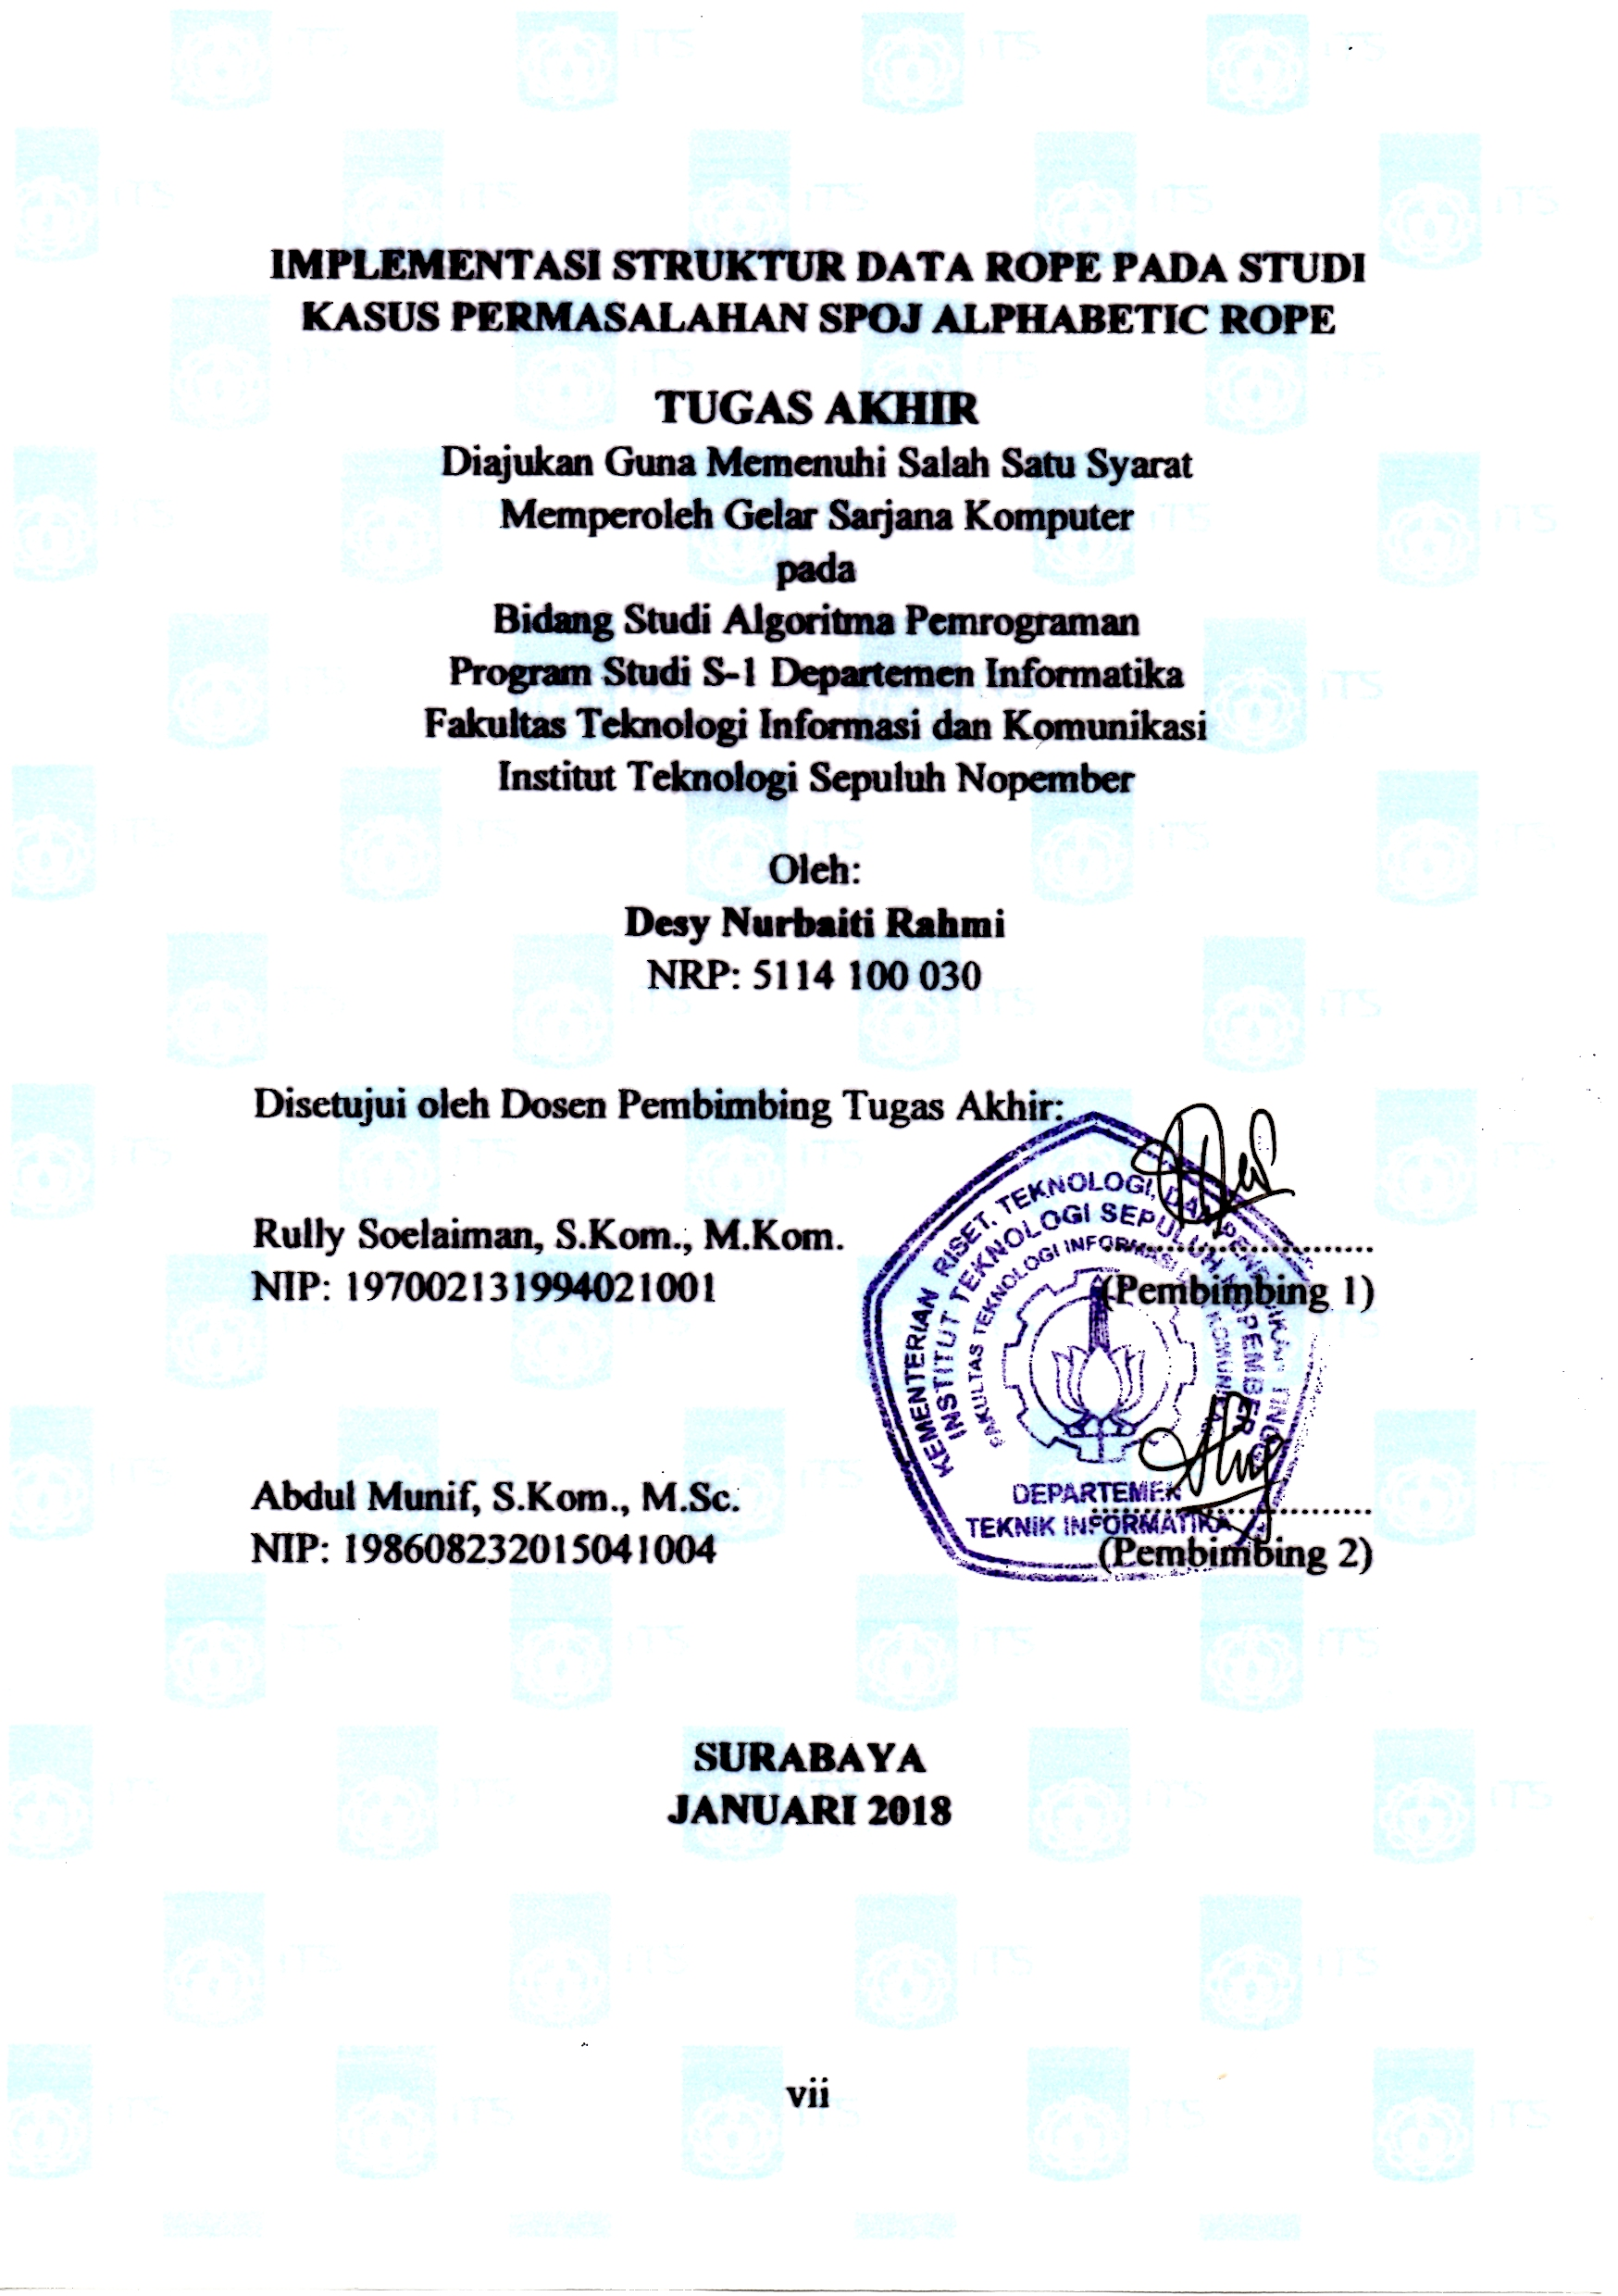
\includegraphics[scale=1]{pengesahan/pengesahan.jpg}}
		\label{figure:lpeng}
	\end{figure}
	
	\cleardoublepage
	% INDONESIAN ABSTRAK
\addcontentsline{toc}{chapter}{ABSTRAK}
\thispagestyle{plain}
\begin{centering}
\textbf{\MakeUppercase{\judul}}
\end{centering}

\begin{tabular}{ll}
Nama  & : \MakeUppercase{\penulis} \\
NRP & : \nrp \\
Departemen  & : \jurusan FTIF-ITS \\
Pembimbing I  & : \pembimbingSatu \\
Pembimbing II  & : \pembimbingDua
\end{tabular}
\\*[20pt]
\begin{centering}
\textbf{Abstrak}
\end{centering}
\itshape
% BEGIN
\\
\indent 
Permasalahan alphabetic rope merupakan sebuah permasalahan yang melibatkan sebuah rentang pencarian. Tipe query secara umum dibagi menjadi dua yaitu, operasi pencarian dan perubahan. Operasi perubahan pada suatu rentang akan menyebabkan perubahan hasil pencarian selanjutnya. Untuk menangani berbagai permasalahan pada operasi alphabetic rope yang harus dilakukan sehingga dibutuhkan struktur data yang mampu mendukung operasi-operasi tersebut dengan efisien.\\
Pada Tugas Akhir ini akan dirancang penyelesaian permasalahan alphabetic rope antara lain operasi pencarian karakter pada indeks ke-y pada konfigurasi rope saat ini, operasi memotong segmen rope pada indeks ke-x sampai y dan menggabungkan pada bagian depan rope, dan operasi memotong segmen rope pada indeks ke-x sampai y dan menggabungkan pada bagian belakang rope. Struktur data klasik yang biasa digunakan dalam penyelesaian permasalahan ini adalah stuktur data String. Namun penggunaan algoritma String masih kurang efisien dalam hal kecepatan dan kebutuhan memori.\\
Pada Tugas Akhir ini digunakan struktur data Rope untuk menyelesaikan operasi-operasi tersebut. Hasil uji coba menunjukkan program menghasilkan jalur yang benar dan memiliki pertumbuhan waktu secara logaritmik dengan kompeksitas waktu sebesar $O(\log N)$ per query.
% END
\rm \\
\textbf{Kata Kunci: concatenation, rope, split, string}


\cleardoublepage

% ENGLISH ABSTRACT
\addcontentsline{toc}{chapter}{ABSTRACT}
\thispagestyle{plain}
\begin{centering}
\textbf{\MakeUppercase{\judulEnglish}}
\end{centering}

\begin{tabular}{ll}
Name  & : \MakeUppercase{\penulis} \\
NRP & : \nrp \\
Major  & : \jurusanEnglish Faculty of IT-ITS \\
Supervisor I  & : \pembimbingSatu \\
Supervisor II  & : \pembimbingDua
\end{tabular}
\\*[20pt]
\begin{centering}
\textbf{Abstract}
\end{centering}
\itshape
% BEGIN
\\
\indent 
Alphabetic rope computation is a problem which involves a specific range of data. Generally it divide by two type of query, range search and update. An update operation would have an impact for the following range search query. To handle various problem in alphabetic rope, an efficient data structure is needed to support the operations.\\
This undergraduate thesis will be designed problem solving for alphabetic rope query variation such as find the y-th position on current rope, cut the rope segment from x-th to y-th to join at the front of rope and cut the rope segment from x-th to y-th and join at the back of rope. Well known data structures, e.g string are commonly used for solving the this problem. But those algorithm were not efficient enough in the term of running time and memory usage.\\
In this undergraduate thesis Rope data structure will be used instead for solving those alphabetic rope variations. The program had been tested and proved that it produces correct result and running in $O(\log N)$ per query.
\\
% END
\rm \\
\textbf{Keywords: concatenation, rope, split, string}

\cleardoublepage

	%\include{istilah/istilah}
	\chapter{KATA PENGANTAR}

\indent\indent Puji syukur Penulis panjatkan kepada Allah SWT. atas pimpinan, penyertaan, dan karunia-Nya sehingga Penulis dapat menyelesaikan Tugas Akhir yang berjudul :
\begin{center}
	\textbf{\MakeUppercase{\judul}}.
\end{center}

Penelitian Tugas Akhir ini dilakukan untuk memenuhi salah satu syarat meraih gelar Sarjana di Departemen Informatika Fakultas Teknologi Informasi dan Komunikasi Institut Teknologi Sepuluh Nopember.

Dengan selesainya Tugas Akhir ini diharapkan apa yang telah dikerjakan Penulis dapat memberikan manfaat bagi perkembangan ilmu pengetahuan terutama di bidang teknologi informasi serta bagi diri Penulis sendiri selaku peneliti.

Penulis mengucapkan terima kasih kepada semua pihak yang telah memberikan dukungan baik secara langsung maupun tidak langsung selama Penulis mengerjakan Tugas Akhir maupun selama menempuh masa studi antara lain:

\begin{itemize}
	\item Bapak, Mama, Ghina dan keluarga Penulis yang selalu memberikan perhatian, dorongan dan kasih sayang yang menjadi semangat utama bagi diri Penulis sendiri baik selama Penulis menempuh masa perkuliahan maupun pengerjaan Tugas Akhir ini.
	\item Bapak Royyana Muslim I., S.Kom., M.Kom., Ph.D. selaku Dosen Pembimbing yang telah banyak meluangkan waktu untuk memberikan ilmu, nasihat, motivasi, pandangan dan bimbingan kepada Penulis baik selama pengerjaan Tugas Akhir ini.
	\item Ibu Henning Titi C., S.Kom., M.Kom. selaku dosen pembimbing yang telah memberikan ilmu, dan masukan kepada Penulis.
	\item Seluruh tenaga pengajar dan karyawan Departemen Informatika ITS yang telah memberikan ilmu dan waktunya demi berlangsungnya kegiatan belajar mengajar di Departemen Informatika ITS.
	\item Seluruh teman angkatan 14 di Departemen Informatika ITS yang telah memberikan dukungan dan semangat kepada Penulis selama Penulis menyelesaikan Tugas Akhir ini.
	\item Teman-teman, kakak-kakak dan adik-adik \textit{administrator} Workshop Pemrograman 2 yang selalu menjadi teman untuk berbagi ilmu.
\end{itemize}

Penulis mohon maaf apabila masih ada kekurangan pada Tugas Akhir ini. Penulis juga mengharapkan kritik dan saran yang membangun untuk pembelajaran dan perbaikan di kemudian hari. Semoga melalui Tugas Akhir ini Penulis dapat memberikan kontribusi dan manfaat yang sebaik-baiknya. \\ \\ \\

\hfill Surabaya, Mei \tahun \\ \\ \\

\hfill \penulis \\
\cleardoublepage

	\tableofcontents
	\cleardoublepage
	\listoftables
	\cleardoublepage
	\listoffigures
	\cleardoublepage
	\lstlistoflistings
	\cleardoublepage
	
	\mainmatter
	\chapter{PENDAHULUAN}
\tab Pada bab ini akan dijelaskan latar belakang, rumusan masalah, batasan masalah, tujuan, manfaat, metodologi dan sistematika penulisan Tugas Akhir.

\section{Latar Belakang}
\tab \textit{Monitoring} adalah suatu kegiatan yang meliputi observasi dan pengecekan terhadap kemajuan suatu proses atau kualitas dari suatu barang atau pekerjaan dan dilakukan secara berkala. Banyak hal yang bisa dimonitor, mulai dari barang, kesehatan, hingga pekerjaan. Untuk keperluan Tugas Akhir ini, \textit{monitoring} dilakukan terhadap perangkat yang ada di Pusat Data Institut Teknologi Sepuluh Nopember (ITS) Surabaya, yakni server dan komputer \textit{single-board}. Tujuan dari adanya \textit{monitoring} ini adalah untuk memantau jaringan dan lingkungan di Pusat Data ITS.\\
\tab \textit{Monitoring} server adalah kegiatan memantau sebuah server dari segi kinerja perangkat keras, \textit{traffic} lalu lintas data, dan masih banyak lagi. \textit{Monitoring} server ini merupakan suatu pekerjaan yang sangat penting untuk dilakukan dalam memanajemen jaringan. \textit{Monitoring} ini menjadi suatu titik yang menentukan apakah suatu layanan jaringan sudah berjalan dengan baik atau tidak.\\
\tab Dalam suatu kegiatan \textit{monitoring} server, tidak semua pengguna layanan bisa melakukan hal tersebut karena terkait dengan hak akses masing-masing. Dan dalam pelaksanaannya selama ini, \textit{monitoring} server dilakukan secara manual dan tidak seragam. Hal ini yang menyebabkan administrator merasa kesulitan dalam mengatasi masalah jaringan yang terjadi.\\
\tab Selain itu, lingkungan di Pusat Data ITS juga perlu dipantau. Amat sulit rasanya jika administrator harus memantau dari komputer \textit{single-board} secara manual. Pekerjaan ini membutuhkan ekstra waktu. Dan belum tentu juga administrator langsung mengetahui jika ada server yang \textit{down} atau keadaan lain yang membutuhkan penanganan langsung.\\
\tab Berdasarkan uraian di atas maka dapat dilihat bahwa dibutuhkan sebuah sistem untuk menangani masalah \textit{monitoring} perangkat yang ada di Pusat Data ITS ini. Dengan adanya sistem yang seragam, diharapkan dapat membantu para administrator dalam memantau server dan komputer \textit{single-board} dengan lebih mudah dan efisien.


\section{Rumusan Masalah}
Rumusan masalah yang diangkat dalam Tugas Akhir ini adalah sebagai berikut:
\begin{enumerate}
	\item Bagaimana cara membangun sistem administrasi \textit{monitoring} untuk pemantauan server?
	\item Bagaimana cara mengimplementasikan \textit{publish-subscribe} pada monitoring server?
	\item Bagaimana cara membangun \textit{agent} yang melaporkan keadaan server ke pengguna?
	\item Bagaimana cara mengambil informasi penggunaan CPU, memori, \textit{bandwidth}, dan hal-hal lain yang terkait pada server?
	\item Bagaimana cara mengimplementasikan \textit{publish-subscribe} pada komputer papan tunggal (\textit{single board computer}) untuk pemantauan lingkungan Pusat Data ITS?
	\item Bagaimana cara mengintegrasikan antara \textit{agent} ke Telegram untuk mengirim notifikasi mengenai keadaan lingkungan atau server di Pusat Data ITS yang membutuhkan penanganan langsung?
\end{enumerate}

\section{Batasan Masalah}
Permasalahan yang dibahas pada Tugas Akhir ini memiliki beberapa batasan, yaitu sebagai berikut:

\begin{enumerate}
	\item Sistem hanya melakukan \textit{monitoring} pada Linux Server dan Raspberry Pi sebagai komputer \textit{single-board} untuk membaca sensor.
	\item Sistem ini diimplementasikan di Pusat Data Institut Teknologi Sepuluh Nopember (ITS) Surabaya.
\end{enumerate}

\section{Tujuan}
Tujuan dari Tugas Akhir ini adalah sebagai berikut:

\begin{enumerate}
	\item Membuat sebuah sistem \textit{monitoring} untuk perangkat di Pusat Data ITS berupa server dan komputer \textit{single-board} yang seragam untuk seluruh pengguna.
	\item Mengimplementasikan metode \textit{publish-subscribe} pada sistem \textit{monitoring} server dan komputer \textit{single-board} di Pusat Data ITS.
\end{enumerate}

\section{Manfaat}
Manfaat dari Tugas Akhir ini adalah sebagai berikut:

\begin{enumerate}
	\item Membangun sebuah sistem administrator \textit{monitoring} server dan komputer \textit{single-board} agar memudahkan para admin dalam memantau server yang ada.
	\item Membangun sistem administrator untuk memantau lingkungan Pusat Data ITS dengan sensor yang dihubungkan ke Raspberry Pi.
	\item Memonitoring server dan yang hanya ingin dimonitoring dengan cara memilih saluran server yang ada.
	\item Membangun \textit{agent} dengan sistem \textit{publish-subscribe} agar dapat melaporkan keadaan server ke pengguna.
	\item Membangun \textit{agent} untuk diletakkan di komputer \textit{single-board} agar bisa melaporkan keadaan lingkungan Pusat Data ITS ke pengguna dengan mengimplementasikan \textit{publish-subscribe}.
	\item Mengetahui informasi seperti penggunaan CPU, memori, \textit{bandwidth}, dan hal lain yang terkait pada server dengan adanya sistem \textit{monitoring} server ini.
	\item Memberitahu pengguna tentang keadaan server atau lingkungan Pusat Data ITS yang butuh perhatian langsung melalui aplikasi Telegram.
\end{enumerate}

\section{Metodologi}
Metodologi yang digunakan dalam pengerjaan Tugas Akhir ini adalah sebagai berikut:
\begin{enumerate}
	
	\item Penyusunan proposal Tugas Akhir
	
	\tab Tahap awal untuk memulai pengerjaan Tugas Akhir adalah penyusunan proposal Tugas Akhir yang berisi gagasan untuk menyelesaikan permasalahan di Pusat Data ITS Surabaya.\\
	\tab Proposal tugas akhir ini berisi tentang deskripsi pendahuluan dari tugas akhir yang akan dibuat. Pendahuluan ini terdiri atas hal yang menjadi latar belakang diajukannya usulan tugas akhir, rumusan masalah yang diangkat, batasan masalah untuk tugas akhir, tujuan dari pembuatan tugas akhir, dan manfaat dari hasil pembuatan tugas akhir. Selain itu dijabarkan pula tinjauan pustaka yang digunakan sebagai referensi pendukung pembuatan tugas akhir. Sub bab metodologi berisi penjelasan mengenai tahapan penyusunan tugas akhir mulai dari penyusunan proposal hingga penyusunan buku tugas akhir. Terdapat pula sub bab jadwal kegiatan yang menjelaskan jadwal pengerjaan tugas akhir.
	
	\item Studi literatur
	
	\tab Pada tahap ini dilakukan pencarian informasi dan studi literatur mengenai pengetahuan atau metode yang dapat digunakan dalam penyelesaian masalah. Informasi didapatkan dari materi-materi yang akan diperlukan untuk membangun aplikasi yaitu mengenai \textit{monitoring} server, Raspberry Pi, dan \textit{Publish-Subscribe}. Materi-materi tersebut didapatkan dari jurnal dan internet.
	
	\item Analisis dan Desain Perangkat Lunak
	
	\tab Pada tahap ini dilakukan analisis dan desain rancangan sistem \textit{monitoring} perangkat di Pusat Data ITS Surabaya.\\
	Aktor dari aplikasi ini adalah administrator yang akan melakukan \textit{monitoring} server dan komputer \textit{single-board}. Admin memilih server atau perangkat mana yang ingin ia pantau. Dari permintaan tersebut, maka sistem akan memberikan informasi perangkat terpilih kepada pengguna yang memilih perangkat tersebut.
	
	\item Implementasi perangkat lunak
	
	\tab Pada tahap ini dilakukan implementasi atau realiasi dari rancangan desain sistem \textit{monitoring} perangkat Pusat Data ITS yang telah dibangun pada tahap desain ke dalam bentuk program.
	
	\item Uji coba dan evaluasi
	
	\tab Pada tahap ini dilakukan uji coba kebenaran implementasi. Pengujian dalam aplikasi ini akan dilakakukan dalam beberapa cara, antara lain:
	\begin{itemize}
		\item Pengujian pada keberhasilan dalam mengambil informasi dari tiap-tiap server (\textit{monitoring} server).
		\item Pengujian pada keberhasilan dalam pengambilan informasi dari komputer \textit{single-board} untuk memantau lingkungan Pusat Data ITS.
		\item Pengujian ini berfokus pada ketepatan informasi dari hasil \textit{monitoring} perangkat dan diberikan (\textit{publish}) ke pengguna yang meminta (\textit{subscribe}).
	\end{itemize}
	
	\item Penyusunan buku Tugas Akhir
	
	Pada tahap ini dilakukan penyusunan buku Tugas Akhir yang berisi dokumentasi hasil pengerjaan Tugas Akhir.
\end{enumerate}

	\section{Sistematika Penulisan}
	Berikut adalah sistematika penulisan buku Tugas Akhir ini:
	\begin{enumerate}
		\item BABI: PENDAHULUAN
		
		Bab ini berisi latar belakang, rumusan masalah, batasan masalah, tujuan, manfaat, metodologi dan sistematika penulisan Tugas Akhir.
		
		\item BAB II: DASAR TEORI
		
		Bab ini berisi dasar teori mengenai permasalahan dan algoritma penyelesaian yang digunakan dalam Tugas Akhir
		
		\item BAB III: DESAIN
		
		Bab ini berisi desain algoritma dan struktur data yang digunakan dalam penyelesaian permasalahan.
		
		\item BAB IV: IMPLEMENTASI
		
		Bab ini berisi implementasi berdasarkan desain algortima yang telah dilakukan pada tahap desain.
		
		\item BAB V: UJI COBA DAN EVALUASI
		
		Bab ini berisi uji coba dan evaluasi dari hasil implementasi yang telah dilakukan pada tahap implementasi.
		
		\item BAB VI: PENUTUP
		
		Bab ini berisi kesimpulan dan saran yang didapat dari hasil uji coba yang telah dilakukan.
	\end{enumerate}

\cleardoublepage

	\chapter{DASAR TEORI}
Pada bab ini akan dijelaskan mengenai dasar teori yang menjadi dasar pengerjaan Tugas Akhir ini.

\section{Deskripsi Permasalahan} \label{section:deskripsi_permasalahan}
Terdapat sebuah \textit{alphabetic rope}\cite{arope} yang terdiri dari karakter-karakter yang terlihat seperti serangkaian \textit{string} dengan karakter yang terdiri dari huruf kecil. Diberikan beberapa operasi perubahan dan atau pertanyaan. Tabel \ref{tab:tipeoperasi} adalah macam-macam tipe operasi pada \problem{}.
\begin{table}[H]
\centering
\begin{tabular}{|p{1cm}|p{8cm}|}
	\hline
	\textbf{$1$ X Y} & Memotong segmen \textit{rope} dari indeks ke-X sampai Y dan menggabungkan pada bagian depan \textit{rope}\\ \hline
	\textbf{$2$ X Y} & Memotong segmen \textit{rope} dari indeks ke-X sampai Y dan menggabungkan pada bagian belakang \textit{rope}\\ \hline
	\textbf{$3$ Y} & Mencetak pada baris baru huruf pada indeks ke-Y dari konfigurasi \textit{rope} saat ini\\ \hline
\end{tabular}
\caption{Tipe Operasi pada Permasalahan \textit{Alphabetic Rope} \label{tab:tipeoperasi}}
\end{table}


\section{Deskripsi Umum}
\tab Pada subbab ini akan dijelaskan mengenai deskripsi-deskripsi umum yang terdapat pada Tugas Akhir ini.

\subsection{SNMP}
\tab SNMP (\textit{Simple Network Management Protocol}) adalah metode “tanpa agen” untuk memonitor perangkat dan server jaringan. Ribuan perangkat jaringan dan sistem operasi yang berbeda dari vendor yang berbeda mendukung SNMP untuk menyampaikan informasi penting yang berhubungan dengan penggunaan, status layanan, dan lainnya.\\
\tab SNMP merupakan pembaharuan dari versi sebelumnya, yakni SGMP (\textit{Simple Gateway Management Protocol}). Protokol ini direncanakan melakukan pertukaran dengan arsitektur \textit{Common Management Information Service/Protocol} (CMIS / CMIP) berdasarkan solusi.\\
\tab SNMP terdiri dari model manajer/agen yang di dalamnya terdapat manajer SNMP, agen MP dan database informasi manajemen, perangkat SNMP yang dikelola dan protokol jaringan. Manajer SNMP menyediakan antarmuka antara manajer jaringan manusia dan sistem manajemen. Agen SNMP menyediakan antarmuka antara manajer dan perangkat fisik yang sedang dikelola.


\subsection{\textit{Publish-Subscribe}}
\tab Secara umum, maksud dari \textit{publish-subscribe} adalah susunan dari sekumpulan node yang didistribusikan melalui jaringan komunikasi. Klien dari sistem ini dibagi menjadi dua peran yaitu \textit{publisher} dan \textit{subscriber}.\\
\tab \textit{Publisher} adalah yang penyedia informasi dan memberikannya kepada yang meminta informasi tersebut. Sedangkan \textit{subscriber} bertindak sebagai konsumen informasi tersebut. Dua klien ini tidak diharuskan untuk berkomunikasi secara langsung di antara mereka sendiri yang namun agak terpisah: interaksi terjadi melalui nodes sistem \textit{publish-subscribe}, yang mengkoordinasikan diri mereka untuk mengarahkan informasi dari penerbit ke pelanggan. Pengunaan \textit{publisher} dan \textit{subscriber} ini dapat memungkinkan skalabilitas yang lebih besar dan topologi jaringan yang lebih dinamis.\\
\tab Terdapat dua jenis \textit{publish-subscribe}, yaitu \textit{topic based} \textit{publish-subscribe} dan \textit{content based} \textit{publish-subscribe}. \textit{Topic based} \textit{publish-subscribe} merupakan pola pengiriman pesan \textit{publish-subscribe} dimana penyedia informasi menyampaikan pesan ke konsumen berdasarkan topik yang dipilihnya. \textit{Content based} \textit{publish-subscribe} merupakan pola pengiriman pesan \textit{publish-subscribe} dimana penyedia informasi menyampaikan pesan ke konsumen berdasarkan isi dari pesan yang ada. Pada umumnya pola pengiriman pesan \textit{publish-subscribe} merupakan \textit{topic based}.


\subsection{Raspiberry Pi}
\tab Raspberry Pi adalah salah satu jenis \textit{Single-Board Computer} (SBC) yang bisa digunakan dalam sistem pemantauan. Raspberry Pi merupakan SBC yang memiliki \textit{low-power} dengan ukuran sebesar kartu kredit yang dirilis pada tahun 2012. Alat ini bisa dibilang merupakan alat yang paling populer yang dikembangkan oleh Universitas Cambridge UK untuk kepentingan pendidikan komputasi.\\
\tab Raspberry Pi ini memiliki RAM sebesar $1$ GB, 900 Mhz \textit{quad-core} ARM Cortex A7 CPU, 10/100 Ethernet, dan dihargai sebesar \textdollar35.00. Alat ini dapat digunakan di sistem operasi Linux dan Windows. Selain itu, alat ini banyak diadaptasi untuk berbagai macam aplikasi seperti sensor jaringan nirkabel, robotika, dan UAV.


\subsection{Rabbitmq}
\tab Rabbitmq merupakan perantara (broker) pada pertukaran pesan. Rabbitmq juga biasa disebut \textit{message-oriented middleware}. Rabbitmq mendukung pola pengiriman pesan \textit{publish-subscribe}.\\
\tab Pada arsitektur pola pengiriman pesan \textit{publish-subscribe} yang terdapat di rabbitmq akan sering ditemui istilah-istilah seperti \textit{exchange} dan \textit{queue}. \textit{Exchange} dapat diartikan sebagai persimpangan, sedangkan \textit{queue} dapat diartikan sebagai tempat penyimpanan. Rabbitmq menggunakan istilah \textit{producer} untuk pihak yang membuat pesan untuk nantinya dikirim ke broker dan \textit{consumer} untuk pihak yang nantinya akan menerima pesan dari broker yang dibuat oleh \textit{producer}. \textit{Producer} pada pola pengiriman pesan \textit{publish-subscribe} dikenal dengan istilah \textit{publisher} sedangkan \textit{consumer} dikenal dengan istilah \textit{subscriber}.\\
\tab Pada arsitektur pola pengiriman pesan \textit{publish-subscribe} pesan yang dibuat oleh \textit{text}publisher mungkin saja dikonsumsi oleh beberapa \textit{subscriber}. \textit{Publisher} nantinya akan mengirim pesan ke suatu \textit{exchange} yang berada pada broker, akan tetapi \textit{exchange} tidak dapat menyimpan pesan. Ketika suatu \textit{exchange} yang dikirimi pesan tidak memiliki \textit{queue} yang tersambung, maka pesan tersebut akan hilang. Pada kasus ini masing-masing \textit{subscriber} akan membuat \textit{queue} yang berbeda untuk menyimpan pesan yang dibuat oleh \textit{publisher}. Oleh rabbitmq pesan yang sudah pernah dipakai (\textit{consume}) akan langsung dihapus dari \textit{queue}.


\subsection{Telegram}
\tab Telegram adalah aplikasi untuk \textit{chatting} yang fokus pada kecepatan dan keamanan. Aplikasi ini tidak berbayar atau gratis. Kelebihan dari Telegram adalah kita dapat membuka akun kita di banyak perangkat secara bersamaan karena pesan akan disinkronisasi dengan baik di sejumlah ponsel, tablet, atau komputer kita.\\
\tab Telegram juga memiliki API yang memperbolehkan pengguna untuk membuat klien Telegram yang disesuaikan dengan pengguna tersebut. API ini gratis untuk siapa saja yang ingin membuat aplikasi Telegram di \textit{platform} ini. Telegram sudah menyediakan \textit{open source code} untuk aplikasi Telegram yang sudah ada agar pengguna bisa melihat bagaimana segala sesuatunya bekerja di sini.
	\chapter{DESAIN}
\label{chapter:desain}

\tab Pada bab ini akan dibahas tentang dasar perancangan sistem yang akan dibuat. Secara khusus akan dibahas mengenai deskripsi umum sistem, perancangan skenario dan arsitektur
sistem.

\section{Deskripsi Umum Sistem}
\tab Tugas akhir ini disusun untuk menangani masalah \textit{monitoring} server dan \textit{computer single-board} dengan menggunakan pola \textit{publish-subscribe}. Pola ini dipilih agar pengguna dapat memilih perangkat mana yang ingin dipantau sehingga tidak semua perangkat terpantau oleh semua orang.\\
\tab Proses \textit{monitoring} ini diawali dengan pengambilan informasi tiap-tiap server menggunakan SNMP \textit{monitoring tools}. Untuk komputer \textit{single-board} diberikan \textit{agent} untuk mengambil data hasil pemantauan. Kemudian pengguna, atau di sini dapat disebutkan sebagai administrator jaringan, dapat memilih saluran (\textit{subscribe}) \textit{server} atau komputer \textit{single-board} mana yang ingin ia pantau melalui sebuah \textit{agent} yang berupa \textit{web-socket}.\\ 
\tab Kemudian, \textit{agent} yang berupa web yang responsif ini akan melanjutkan permintaan ke sebuah \textit{middleware}. \textit{Middleware} yang telah terpola \textit{publish-subscribe} ini akan memproses permintaan tersebut. Kemudian perangkat yang terpilih akan memberikan informasinya (\textit{publish}) melalui \textit{middleware} dan diteruskan kembali ke \textit{agent} berupa notifikasi. Notifikasi ini dapat dilihat oleh admin. Selain itu, \textit{agent} juga mengirimkan notifikasi mengenai keadaan lingkungan dan \textit{server} Pusat Data ITS yang butuh penanganan langsung, seperti \textit{server time out}, suhu ruangan meningkat tajam, ke Telegram. Sehingga administrator bisa langsung bertindak cepat.

\section{Perancangan}
skjsdfbavekdnhkdfsnkd

\section{Arsitektur Sistem}
kljfnksjfjsklj

	\chapter{IMPLEMENTASI}
\label{chapter:implementasi}

Pada bab ini dijelaskan mengenai implementasi dari desain dan algoritma penyelesaian \problem{}.

\section{Lingkungan Implementasi}
Lingkungan implementasi dalam pembuatan Tugas Akhir ini meliputi perangkat keras dan perangkat lunak yang digunakan untuk penyelesaian \problem{} adalah sebagai berikut:

\begin{enumerate}
	\item Perangkat Keras:
		\begin{itemize}
			\item \textit{Processor} Intel(R) Core(TM) i3 - M 330 CPU @ 2.13GHz x 4 \item Memori 4 GB.
		\end{itemize}
	\item Perangkat Lunak:
	\begin{itemize}
		\item Sistem operasi Ubuntu 14.04 LTS 64 bit.
		\item \textit{Text editor} Sublime Text 3.
		\item \textit{Compiler} g++ versi 4.3.2.
	\end{itemize}			
\end{enumerate}


\section{Rancangan Data}
Pada subbab ini dijelaskan mengenai desain data masukan yang diperlukan untuk melakukan proses algoritma, dan data keluaran yang dihasilkan oleh program.

\subsection{Data Masukan}
Data masukan adalah data yang akan diproses oleh program sebagai masukan menggunakan algoritma dan struktur data yang telah dirancang dalam Tugas Akhir ini.\\
Data masukan berupa berkas teks yang berisi data dengan format yang telah ditentukan pada deskripsi \problem{}. Pada masing-masing berkas data masukan, baris pertama berupa sebuah bilangan bulat yang merepresentasikan jumlah kasus uji yang ada pada berkas tersebut. Untuk setiap kasus uji dengan tipe $1$ dan $2$, masukan berupa sebuah baris masukan yang terdiri dari dua buah parameter posisi berupa $x$ dan $y$. Sedangkan pada kasus uji dengan tipe $3$, masukan berupa sebuah parameter $y$ yang merupakan indeks \textit{string} yang dicari pada konfigurasi \textit{rope} saat ini.

\subsection{Data Keluaran}
Data keluaran yang dihasilkan oleh program hanya berupa satu nilai, yaitu huruf pada indeks ke-$y$ untuk setiap kasus uji dengan tipe $3$. 

\section{Implementasi Algoritma}
Pada subbab ini akan dijelaskan tentang implementasi proses algoritma secara keseluruhan berdasarkan desain yang telah dijelaskan pada Bab \ref{chapter:desain}.

\subsection{\textit{Header} yang Diperlukan}
Implementasi algoritma dengan pemanfaatan struktur data Rope untuk menyelesaikan \problem{} membutuhkan empat buah \textit{header} yaitu stdio.h, cstdlib, cstring dan utility, seperti yang terlihat pada Kode Sumber \ref{source:header}.\\

\lstinputlisting[language=C++, firstline=1, lastline=4, caption=\textit{Header} yang diperlukan, label=source:header]{assets/code/include.cpp}

\textit{Header} stdio.h berisi modul untuk menerima masukan dan memberikan keluaran. \textit{Header} cstdlib berisi modul untuk manajemen memori dinamis, generasi bilangan acak, pemilahan dan konversi. \textit{Header} cstring berisi modul yang memiliki fungsi-fungsi untuk melakukan pemrosesan \textit{string}. \textit{Header} utility mencakup berbagai modul yang menyediakan fungsionalitas mulai dari aplikasi perhitungan bit hingga aplikasi fungsi parsial. Contoh implementasinya penggunaan \textit{pair}. 

\subsection{Variabel Global}
Variabel global digunakan untuk memudahkan dalam mengakses data yang digunakan lintas fungsi. Kode sumber implementasi variabel global dapat dilihat pada Kode Sumber \ref{source:variabel_global}.

\begin{minipage}{\linewidth}
\lstinputlisting[language=C++, firstline=1, lastline=3, caption=Variabel Global, label=source:variabel_global]{assets/code/global.cpp}
\end{minipage}
	
\subsection{Implementasi Fungsi Main}
Fungsi Main adalah implementasi algoritma yang dirancang pada Gambar \ref{figure:fungsi_main}. Setiap tipe memiliki operasi yang berbeda-beda. Untuk operasi dengan tipe $3$, masukan hanya berupa parameter $y$ yang merupakan nilai posisi indeks yang dicari pada konfigurasi \textit{rope} saat ini. Pada operasi dengan tipe $1$ dan $2$, baris masukan berupa nilai $x$ dan $y$ yang merupakan posisi indeks dari \textit{string} pada \textit{rope}. Setiap masukan dengan tipe $3$ akan ditampilkan sebagai jawaban akhir dari permasalahan. Implementasi fungsi Main dapat dilihat pada Kode Sumber \ref{source:fungsi_main}.

\lstinputlisting[language=C++, firstline=1, lastline=24, caption=Fungsi Main, label=source:fungsi_main]{assets/code/main.cpp}

\subsection{Implementasi Struct Node}
Fungsi Struct Node berisi atribut yang dimiliki \textit{node} pada \textit{tree}. Implementasi dari fungsi Struct Node dapat dilihat pada Kode Sumber \ref{source:fungsi_struct}.

\lstinputlisting[language=C++, firstline=1, lastline=17, caption=Fungsi Struct Node, label=source:fungsi_struct]{assets/code/struct.cpp}

\subsection{Implementasi Fungsi Newnode}
Fungsi Newnode digunakan untuk membentuk sebuah \textit{node} yang berisikan karakter yang diberikan dan relasi terhadap karakter pada posisi yang bersebelahan. Sehingga membentuk sebuah \textit{tree} seperti pada Gambar \ref{fig:bst}. Implementasi fungsi \proc{newnode} dapat dilihat pada Kode Sumber \ref{source:fungsi_newnode}.

\lstinputlisting[language=C++, firstline=1, lastline=7, caption=Fungsi Newnode, label=source:fungsi_newnode]{assets/code/newnode.cpp}

\subsection{Implementasi Fungsi Build}
Fungsi Build membangun struktur \textit{tree} dari \textit{rope} yang dilakukan dari karakter yang berada pada posisi indeks di tengah sampai pada karakter paling awal maupun akhir.  Setiap \textit{node} akan memiliki anak kiri dan anak kanan jika dan hanya jika masih terdapat \textit{string} yang tersisa. Ilustrasinya dapat dilihat pada Gambar \ref{fig:rope}. Implementasi dari Fungsi Build dapat dilihat pada Kode Sumber \ref{source:fungsi_build}.

\lstinputlisting[language=C++, firstline=1, lastline=6, caption=Fungsi Build, label=source:fungsi_build]{assets/code/build.cpp}

\subsection{Implementasi Fungsi Getsize}
Fungsi Getsize digunakan untuk mendapatkan berat \textit{node} yang diperlukan. Implementasi dari fungsi Getsize dapat dilihat pada Kode Sumber \ref{source:fungsi_getsize}.

\lstinputlisting[language=C++, firstline=1, lastline=3, caption=Fungsi Getsize, label=source:fungsi_getsize]{assets/code/getsize.cpp}

\subsection{Implementasi Fungsi Split}
Fungsi Split memanfaatkan struktur data Pair yang berupa pasangan dari dua \textit{pointer} menuju \textit{node}. \textit{Pointer node} pertama akan berisi semua \textit{node} yang bernilai lebih kecil dari posisi indeks parameter \textit{split}, sedangkan \textit{pointer node} kedua berisi semua \textit{node} yang bernilai lebih besar sama dengan posisi indeks parameter \textit{split}.\\
Misalkan dilakukan \textit{split} pada indeks ke-$5$ dari \textit{rope} pada Gambar \ref{fig:split-5}, \textit{pointer node} pertama akan menyimpan semua \textit{node} dari indeks ke-$0$ sampai dengan $4$. Sedangkan \textit{pointer node} kedua menyimpan \textit{node} dari indeks ke-$5$ sampai akhir. Implementasi dari fungsi \textit{split} dapat dilihat pada Kode Sumber \ref{source:fungsi_split1} dan \ref{source:fungsi_split2}.
\begin{figure}
\centering
\begin{tikzpicture}[level/.style={sibling distance = 8cm/#1, level distance = 1.5cm}, scale=0.6,transform shape]
\node[treenode]{b,12}
  child{
    node[treenode]{t,6} 
    child {
    	node[treenode] {a,3}
    	child {
    		node[treenode]{g,1}
    	}
    	child{
    		node[treenode] {u,1}
    	}
    }
    child {
    	node[treenode] {m,2}
    	child {
    	    node[treenode] {a,1}
    	}
    	child[missing]{}
    }
  }
  child{
  	node[treenode]{h,5}
  	child {
  	    	node[treenode] {s,2}
  	    	child {
  	    		node[treenode]{i,1}
  	    	}
  	    	child[missing]{}
  	    }
  	    child {
  	    	node[treenode] {l,2}
  	    	child {
  	    	    node[treenode] {a,1}
  	    	}
  	    	child[missing] {}
  	    }
  };
  \draw [line width = 1pt] (-2.3,0) -- (-2.3,0) .. controls (-3.5,-2.5) .. (-2.1, -4.8);
\end{tikzpicture}
\begin{tikzpicture}[level/.style={sibling distance = 5cm/#1, level distance = 1.5cm}, scale=0.65,transform shape]
\node{
	\begin{tabular}{|c|c|}
		\hline
		pair first & pair second\\ \hline
	\end{tabular}
}
  child{
    node[treenode]{t,5} 
    child {
    	node[treenode] {a,3}
    	child {
    		node[treenode]{g,1}
    	}
    	child{
    		node[treenode] {u,1}
    	}
    }
    child {
    	node[treenode] {a,1}
    }
  }
  child{
  	node[treenode]{b,7}
  	child {
  		node[treenode]{m,1}
  	}
	child {
		node[treenode]{h,5}
		child {
			node[treenode] {s,2}
		  	child {
	  	   		node[treenode]{i,1}
  	    	}
  	    	child[missing]{}
  	    }
  	    child {
  	    	node[treenode] {l,2}
  	    	child {
  	    	    node[treenode] {a,1}
  	    	}
  	    	child[missing] {}
  	    }
	}
  };
\end{tikzpicture}
\caption{Ilustrasi Penyimpanan Hasil Operasi \textit{Split Rope} pada Struktur Data Pair \label{fig:split-5}}
\end{figure}

\lstinputlisting[language=C++, firstline=1, lastline=5, caption=Fungsi Split(1), label=source:fungsi_split1]{assets/code/split.cpp}
\lstinputlisting[language=C++, firstline=6, lastline=19, caption=Fungsi Split(2), label=source:fungsi_split2]{assets/code/split.cpp}

\subsection{Implementasi Fungsi Random}
Fungsi Random digunakan untuk menentukan posisi \textit{node} pada saat penggabungan dua buah \textit{rope}. Digunakan fungsi Random agar posisi \textit{node} tidak konstan dan berat suatu \textit{rope} tidak selalu sama. Implementasi fungsi Random ditunjukkan pada Kode Sumber \ref{source:fungsi_random}.

\lstinputlisting[language=C++, firstline=1, lastline=3, caption=Fungsi Random, label=source:fungsi_random]{assets/code/random.cpp}

\subsection{Implementasi Fungsi Concate}
Fungsi Concate menggabungkan dua buah \textit{rope} menjadi sebuah \textit{rope} utuh. Untuk setiap \textit{node} yang memiliki hasil modular nilai acak lebih kecil dari berat \textit{node root rope} pertama, akan menjadi \textit{root} dari \textit{rope} yang baru terbentuk. Untuk \textit{rope} kedua akan menjadi anak kanan atau anak kirinya, tergantung pada urutan BST yang seharusnya dibuat.\\
Misalkan terdapat dua buah \textit{rope} $R_1$ yang berisi \textit{string} "$abc$" dan $R_2$ yang berisi \textit{string} "$def$" seperti pada Gambar \ref{fig:concate-ab}. Apabila akan digabungkan dengan $R_1$ berada di posisi depan sehingga membentuk \textit{string} "$abcdef$", maka semua \textit{node} pada $R_2$ berada di posisi kanan rope $R_1$. Jika nilai hasil modular $R_1$ lebih kecil dari berat \textit{node root} $R_1$, \textit{node} tersebut akan menjadi \textit{root} dari \textit{rope} yang baru terbentuk. \textit{Node root} $R_2$ akan menjadi anak kanannya. Jika \textit{root} $R_1$ memiliki anak kanan, akan menjadi anak kiri dari \textit{node} $R_1$ yang memiliki indeks $0$. Implementasi Fungsi Concate ditunjukkan pada Kode Sumber \ref{source:fungsi_concate_1} dan \ref{source:fungsi_concate_2}.
\begin{figure}
\begin{tikzpicture}[level/.style={sibling distance = 5cm/#1, level distance = 1.5cm}, scale=0.65,transform shape]
\node[treenode]{b,3}
  child{
  	node[treenode]{a,1}
  }
  child{
  	node[treenode]{c,1}
  };
\end{tikzpicture}
\begin{tikzpicture}[level/.style={sibling distance = 5cm/#1, level distance = 1.5cm}, scale=0.65,transform shape]
\node[treenode]{e,3}
  child{
  	node[treenode]{d,1}
  }
  child{
  	node[treenode]{f,1}
  };
\end{tikzpicture}
\centerline
{\begin{tikzpicture}[level/.style={sibling distance = 5cm/#1, level distance = 1.5cm}, scale=0.7,transform shape]
\node[treenode]{b,6}
  child{
  	node[treenode]{a,1}
  }
  child{
  	node[treenode]{e,4}
  	child {
  		node[treenode] {d,2}
  		child {
  			node[treenode]{c,1}
  		}
  		child[missing]{}
  	}
  	child {
  		node[treenode] {f,1}
  	}
  };
\end{tikzpicture}}
\caption{Ilustrasi Operasi Concate. Setiap \textit{Node} Berisi Sebuah Karakter dan Nilai Berat Masing-Masing \textit{Node} \label{fig:concate-ab}}
\end{figure}

\lstinputlisting[language=C++, firstline=1, lastline=2, caption=Fungsi Concate(1), label=source:fungsi_concate_1]{assets/code/concate.cpp}

\lstinputlisting[language=C++, firstline=3, lastline=10, caption=Fungsi Concate(2), label=source:fungsi_concate_2]{assets/code/concate.cpp}

\subsection{Implementasi Fungsi Insert}
Fungsi Insert adalah implementasi dari desain algoritma pada Gambar \ref{figure:fungsi_insert}. Fungsi ini bertujuan untuk memasukkan data \textit{string} ke dalam \textit{rope}. Setiap \textit{string} akan dimasukkan ke dalam suatu \textit{node}. Setiap \textit{node} hanya berisi oleh satu karakter pecahan dari \textit{string} masukan. Implementasi dari Fungsi Insert dapat dilihat pada Kode Sumber \ref{source:fungsi_insert}.

\lstinputlisting[language=C++, firstline=1, lastline=4, caption=Fungsi Insert, label=source:fungsi_insert]{assets/code/insert.cpp}

\subsection{Implementasi Fungsi Mutable Begin}
Fungsi Mutable Begin adalah implementasi dari desain algoritma pada Gambar \ref{figure:fungsi_mutable_begin}. Operasi ini dilakukan untuk menjawab permasalahan pada subbab \ref{chapter:operasi1} dengan memanfaatkan dua buah operasi Split dan dua buah operasi Concate.\\
Misal dilakukan operasi $1$ $5$ $9$ pada \textit{rope} di Gambar \ref{fig:mutbegin}. Maka \textit{rope} akan dipotong pada posisi indeks ke-$5$ menghasilkan \textit{rope} $R_1$ dan $R_2$. Kemudian dilakukan \textit{split} kedua kali pada indeks $y-x+1$ pada \textit{rope} $R_2$ menghasilkan \textit{rope} $R_{21}$ dan $R_{22}$. Sehingga menghasilkan tiga buah \textit{rope} yang disimpan dalam struktur data Pair. Langkah selanjutnya dilakukan operasi Concate pada \textit{rope} $R_1$ dengan $R_{22}$. Hasil penggabungan \textit{rope} $R_1$ dengan $R_{22}$ akan digabungkan dengan \textit{rope} $R_{21}$. Pada operasi ini, \textit{rope} $R_{21}$ akan berada di posisi paling kiri dari keseluruhan \textit{rope}. Dan menghasilkan sebuah \textit{rope} utuh dengan urutan posisi \textit{rope} saat ini adalah $R_{21}$, $R_1$ dan $R_{22}$. Implementasi Fungsi Mutable Begin dapat dilihat pada Kode Sumber \ref{source:fungsi_mutable_begin}.
\begin{figure}
\centering
\begin{tikzpicture}[level/.style={sibling distance = 8cm/#1, level distance = 1.5cm}, scale=0.6,transform shape]
\node[splitnode]{b,12}
  child{
    node[treenode]{t,6} 
    child {
    	node[treenode] {a,3}
    	child {
    		node[treenode]{g,1}
    	}
    	child{
    		node[treenode] {u,1}
    	}
    }
    child {
    	node[splitnode] {m,2}
    	child {
    	    node[treenode] {a,1}
    	}
    	child[missing]{}
    }
  }
  child{
  	node[splitnode]{h,5}
  	child {
  	    	node[splitnode] {s,2}
  	    	child {
  	    		node[splitnode]{i,1}
  	    	}
  	    	child[missing]{}
  	    }
  	    child {
  	    	node[treenode] {l,2}
  	    	child {
  	    	    node[treenode] {a,1}
  	    	}
  	    	child[missing] {}
  	    }
  };
  \draw [line width = 1pt] (-2.3,0) -- (-2.3,0) .. controls (-3.5,-2.5) .. (-2.1, -4.8);
\end{tikzpicture}
\centering
\begin{tikzpicture}[level/.style={sibling distance = 5cm/#1, level distance = 1.5cm}, scale=0.68,transform shape]
\node[treenode]{t,5} 
    child {
    	node[treenode] {a,3}
    	child {
    		node[treenode]{g,1}
    	}
    	child{
    		node[treenode] {u,1}
    	}
    }
    child {
    	node[treenode] {a,1}
    };
\end{tikzpicture}
\centering
\begin{tikzpicture}[level/.style={sibling distance = 5cm/#1, level distance = 1.5cm}, scale=0.6,transform shape]
\node[splitnode]{b,7}
  child{
    node[splitnode]{m,1} 
  }
  child{
  	node[splitnode]{h,5}
  	child {
  	    	node[splitnode] {s,2}
  	    	child {
  	    		node[splitnode]{i,1}
  	    	}
  	    	child[missing]{}
  	    }
  	    child {
  	    	node[treenode] {l,2}
  	    	child {
  	    	    node[treenode] {a,1}
  	    	}
  	    	child[missing] {}
  	    }
  };
  \draw[-, line width = 1pt] (3.5,-1.8) -- (1.8,-4.5);
\end{tikzpicture}
\centering
\begin{tikzpicture}[level/.style={sibling distance = 5cm/#1, level distance = 1.5cm}, scale=0.6,transform shape]
\node[treenode]{t,7}
child {
	node[treenode]{a,3}
	child {
		node[treenode]{g,1}
	}
	child {
		node[treenode]{u,2}
	}
}
child {
	node[treenode]{l,3}
	child {
		node[treenode]{a,2}
		child {
			node[treenode]{a,1}
		}
		child[missing]{}
	}
	child[missing] {}
};
\end{tikzpicture}
\centering
\begin{tikzpicture}[level/.style={sibling distance = 3cm/#1, level distance = 1.5cm}, scale=0.55,transform shape]
\node[treenode]{b,5}
child {
	node[treenode]{m,1}
}
child{
	node[treenode]{h,3}
	child {
		node[treenode]{2,s}
		child {
			node[treenode]{i,1}
		}
		child[missing]{}
	}
	child[missing] {}
};
\end{tikzpicture}
\begin{tikzpicture}[level/.style={sibling distance = 5cm/#1, level distance = 1.5cm}, level 2/.style={sibling distance = 2cm}, level 3/.style={sibling distance = 1.5cm}, level 4/.style={sibling distance = 1.5cm}, scale=0.65,transform shape]
\node[treenode]{t,12}
child {
	node[treenode]{b,8}
	child {
		node[treenode]{m,1}
	}
	child {
		node[treenode]{h,6}
		child {
			node[treenode]{s,2}
			child {
				node[treenode]{i,1}
			}
			child[missing]{}
		}
		child {
			node[treenode]{a,3}
			child {
				node[treenode]{g,1}
			}
			child {
				node[treenode]{u,1}
			}
		}
	}
}
child {
	node[treenode]{l,3}
	child {
		node[treenode]{a,2}
		child {
			node[treenode]{a,1}
		}
		child[missing]{}
	}
	child[missing] {}
};
\end{tikzpicture}
\caption{Ilustrasi Operasi Mutable Begin. Setiap \textit{Node} Berisi Sebuah Karakter dan Nilai Prioritas Masing-Masing \textit{Node} \label{fig:mutbegin}}
\end{figure}

\lstinputlisting[language=C++, firstline=1, lastline=6, caption=Fungsi Mutable Begin, label=source:fungsi_mutable_begin]{assets/code/mutable_begin.cpp}

\subsection{Implementasi Fungsi Mutable End}
Fungsi Mutable End dilakukan untuk menjawab permasalahan pada subbab \ref{chapter:operasi2}. Implementasinya dilakukan dengan memanfaatkan dua buah operasi Split dan dua buah operasi Concate.\\
Misal dilakukan operasi $2$ $5$ $9$ pada rope di Gambar \ref{fig:mutend}. Maka \textit{rope} akan dipotong pada posisi indeks ke-$5$ menghasilkan rope $R_1$ dan $R_2$. Kemudian dilakukan \textit{split} kedua kali pada indeks $y-x+1$ pada \textit{rope} $R_2$ menghasilkan \textit{rope} $R_{21}$ dan $R_{22}$. Sehingga menghasilkan tiga buah \textit{rope} yang disimpan dalam struktur data Pair. Langkah selanjutnya dilakukan operasi Concate pada \textit{rope} $R_1$ dengan $R_{22}$. Hasil penggabungan \textit{rope} $R_1$ dengan $R_{22}$ akan digabungkan dengan \textit{rope} $R_{21}$. Pada operasi ini, \textit{rope} $R_{21}$ akan berada di posisi paling kanan dari keseluruhan \textit{rope}. Dan menghasilkan sebuah \textit{rope} utuh dengan urutan posisi \textit{rope} saat ini adalah $R_1$, $R_{22}$ dan $R_{21}$. Implementasi Fungsi Mutable End dapat dilihat pada Kode Sumber \ref{source:fungsi_mutable_end}.
\begin{figure}
\centering
\begin{tikzpicture}[level/.style={sibling distance = 8cm/#1, level distance = 1.5cm}, scale=0.6,transform shape]
\node[splitnode]{b,12}
  child{
    node[treenode]{t,6} 
    child {
    	node[treenode] {a,3}
    	child {
    		node[treenode]{g,1}
    	}
    	child{
    		node[treenode] {u,1}
    	}
    }
    child {
    	node[splitnode] {m,2}
    	child {
    	    node[treenode] {a,1}
    	}
    	child[missing]{}
    }
  }
  child{
  	node[splitnode]{h,5}
  	child {
  	    	node[splitnode] {s,2}
  	    	child {
  	    		node[splitnode]{i,1}
  	    	}
  	    	child[missing]{}
  	    }
  	    child {
  	    	node[treenode] {l,2}
  	    	child {
  	    	    node[treenode] {a,1}
  	    	}
  	    	child[missing] {}
  	    }
  };
  \draw [line width = 1pt] (-2.3,0) -- (-2.3,0) .. controls (-3.5,-2.5) .. (-2.1, -4.8);
\end{tikzpicture}
\centering
\begin{tikzpicture}[level/.style={sibling distance = 5cm/#1, level distance = 1.5cm}, scale=0.68,transform shape]
\node[treenode]{t,5} 
    child {
    	node[treenode] {a,3}
    	child {
    		node[treenode]{g,1}
    	}
    	child{
    		node[treenode] {u,1}
    	}
    }
    child {
    	node[treenode] {a,1}
    };
\end{tikzpicture}
\centering
\begin{tikzpicture}[level/.style={sibling distance = 5cm/#1, level distance = 1.5cm}, scale=0.6,transform shape]
\node[splitnode]{b,7}
  child{
    node[splitnode]{m,1} 
  }
  child{
  	node[splitnode]{h,5}
  	child {
  	    	node[splitnode] {s,2}
  	    	child {
  	    		node[splitnode]{i,1}
  	    	}
  	    	child[missing]{}
  	    }
  	    child {
  	    	node[treenode] {l,2}
  	    	child {
  	    	    node[treenode] {a,1}
  	    	}
  	    	child[missing] {}
  	    }
  };
  \draw[-, line width = 1pt] (3.5,-1.8) -- (1.8,-4.5);
\end{tikzpicture}
\centering
\begin{tikzpicture}[level/.style={sibling distance = 5cm/#1, level distance = 1.5cm}, scale=0.6,transform shape]
\node[treenode]{t,7}
child {
	node[treenode]{a,3}
	child {
		node[treenode]{g,1}
	}
	child {
		node[treenode]{u,2}
	}
}
child {
	node[treenode]{l,3}
	child {
		node[treenode]{a,2}
		child {
			node[treenode]{a,1}
		}
		child[missing]{}
	}
	child[missing] {}
};
\end{tikzpicture}
\centering
\begin{tikzpicture}[level/.style={sibling distance = 3cm/#1, level distance = 1.5cm}, scale=0.55,transform shape]
\node[treenode]{b,5}
child {
	node[treenode]{m,1}
}
child{
	node[treenode]{h,3}
	child {
		node[treenode]{2,s}
		child {
			node[treenode]{i,1}
		}
		child[missing]{}
	}
	child[missing] {}
};
\end{tikzpicture}
\begin{tikzpicture}[level/.style={sibling distance = 5cm/#1, level distance = 1.5cm}, level 2/.style={sibling distance = 3cm}, level 3/.style={sibling distance = 1.5cm}, level 4/.style={sibling distance = 1.5cm}, scale=0.65,transform shape]
\node[treenode]{b,12}
child {
	node[treenode]{t,8}
	child {
		node[treenode]{a,3}
		child {
			node[treenode]{g,1}
		}
		child {
			node[treenode]{u,1}
		}
	}
	child {
		node[treenode]{m,4}
		child {
			node[treenode]{l,3}
			child {
				node[treenode]{a,2}
				child {
					node[treenode]{a,1}
				}
				child[missing]{}
			}
			child[missing]{}
		}
		child[missing]{}
	}
}
child {
	node[treenode]{h,3}
	child {
		node[treenode]{s,2}
		child {
			node[treenode]{i,1}
		}
		child[missing]{}
	}
	child[missing] {}
};
\end{tikzpicture}
\caption{Ilustrasi Operasi Mutable End. Setiap \textit{Node} Berisi Sebuah Karakter dan Nilai Prioritas Masing-Masing \textit{Node} \label{fig:mutend}}
\end{figure}
\lstinputlisting[language=C++, firstline=1, lastline=6, caption=Fungsi Mutable End, label=source:fungsi_mutable_end]{assets/code/mutable_end.cpp}

\subsection{Implementasi Fungsi Print}
Fungsi Print digunakan untuk menjawab \problem{} sesuai dengan permasalahan pada subbab \ref{chapter:operasi3}. Implementasi fungsi ini berdasarkan dari desain algorithma pada Gambar \ref{figure:fungsi_print}. Implementasi dari Fungsi Print dapat dilihat pada Kode Sumber \ref{source:fungsi_print}.

\lstinputlisting[language=C++, firstline=1, lastline=6, caption=Fungsi Print, label=source:fungsi_print]{assets/code/print.cpp}
	\chapter{UJI COBA DAN EVALUASI}

Pada bab ini dijelaskan tentang uji coba dan evaluasi dari implementasi yang telah dilakukan pada Tugas Akhir ini.

\section{Lingkungan Uji Coba}

Linkungan uji coba yang digunakan adalah salah satu sistem yang digunakan situs penilaian daring SPOJ, yaitu kluster \textit{Cube} dengan spesifikasi sebagai berikut:

\begin{enumerate}
	\item Perangkat Keras:
	\begin{itemize}
		\item \textit{Processor} Intel(R) Pentium G860 CPU @ 3GHz.
		\item \textit{Memory} 1536 MB.
	\end{itemize}
	\item Perangkat Lunak:
	\begin{itemize}
		\item \textit{Compiler} g++ versi 4.3.2.
	\end{itemize}			
\end{enumerate} 

\section{Uji Coba Kebenaran}
\label{section:ujikebenaran}
Uji coba kebenaran dilakukan dengan analisis penyelesaian sebuah contoh kasus menggunakan pendekatan penyelesaian yang telah dijelaskan pada subbab \ref{chapter:rope} serta pengumpulan berkas kode sumber hasil implementasi ke dalam situs penilaian daring SPOJ.\\
Kasus yang akan digunakan sebagai bahan uji kebenaran dalam analisis penyelesaian \problem{} menggunakan contoh kasus pada Gambar \ref{figure:sample_problem}.
\begin{figure}[h]
	%\inputminted[frame=lines]{text}{bab5/rope.in} %
	\begin{tikzpicture}
	\node (example-align) [draw, text width=10cm, align=left, font=\ttfamily]{gautambishal \\3\\3 1\\2 0 5\\3 1};
	\end{tikzpicture}
	\caption{Contoh kasus uji permasalahan Alphabetic Rope}
	\label{figure:sample_problem}
\end{figure}\\
Mula-mula dalam setiap permasalahan adalah membangun struktur \textit{rope} yang sesuai dengan \textit{string} masukan. Operasi dasar pada sebuah \textit{rope} adalah fungsi Insert, dimana dibentuk sebuah \textit{tree} yang berfungsi untuk menyimpan potongan karakter pada \textit{rope}. Selanjutnya \textit{rope} akan dibangun pada \textit{node root} yang dilakukan berdasarkan posisi tengah dari panjang \textit{string}. Pembentukan ini dapat dilihat pada Gambar \ref{fig:build_root}. Nilai pada tanda kurung siku menyatakan isi karakter pada \textit{node} tersebut. Dikarenakan masih terdapat \textit{string} yang tersisa maka proses pembentukan dilanjutkan untuk membentuk anak kiri dan anak kanan \textit{root}.
\begin{figure}[h]
\centering
\begin{tikzpicture}[->,>=stealth', level/.style={sibling distance = 5cm/#1, level distance = 1.5cm}, scale=0.93,transform shape]
\node {
	[b]
	\begin{tabular}{|c|c|c|c|c|c|c|c|c|c|c|c|}
		\hline
		g & a & u & t & a & m & b & i & s & h & a & l\\ \hline
		\nc{0} & \nc{1} & \nc{2} & \nc{3} & \nc{4} & \nc{5} & \nc{6} & \nc{7} & \nc{8} & \nc{9} & \nc{10} & \nc{11}\\
	\end{tabular}
};
\end{tikzpicture}
\caption{Pembentukan \textit{Root Rope} \label{fig:build_root}}
\end{figure}
Rentang \textit{string} pada anak kiri diperoleh dari indeks $0$ hingga nilai tengah$-1$ sedangkan rentang kanan diperoleh dari nilai tengah$+1$ hingga panjang \textit{string}. Pembentukan anak dari \textit{root} ditunjukkan pada Gambar \ref{fig:build_level1}. Pada setiap anak kiri dan anak kanan, posisi karakter yang berada ditengah-tengah \textit{string} anak menjadi nilai dari \textit{node} tersebut. Yang ditunjukkan oleh nilai di dalam tanda kurung siku.
\begin{figure}[h]
\centering
\begin{tikzpicture}[->,>=stealth', level/.style={sibling distance = 5cm/#1, level distance = 1.5cm}, scale=0.93,transform shape]
\node {
	[b]
	\begin{tabular}{|c|c|c|c|c|c|c|c|c|c|c|c|}
		\hline
		g & a & u & t & a & m & b & i & s & h & a & l\\ \hline
		\nc{0} & \nc{1} & \nc{2} & \nc{3} & \nc{4} & \nc{5} & \nc{6} & \nc{7} & \nc{8} & \nc{9} & \nc{10} & \nc{11}\\
	\end{tabular}
}
child {
	node {
		[t]
		\begin{tabular}{|c|c|c|c|c|c|}
			\hline
			g & a & u & t & a & m\\ \hline
			\nc{0} & \nc{1} & \nc{2} & \nc{3} & \nc{4} & \nc{5}\\
		\end{tabular}
	}
} 
child {
	node {
		[h]
		\begin{tabular}{|c|c|c|c|c|}
			\hline
			i & s & h & a & l\\ \hline
			\nc{7} & \nc{8} & \nc{9} & \nc{10} & \nc{11}\\
		\end{tabular}
	}
};
\end{tikzpicture}
\caption{Pembentukan \textit{Rope} pada Tingkat ke-$2$ \label{fig:build_level1}}
\end{figure}\\
Dikarenakan masih terdapat \textit{string} yang tersisa, proses pembentukan dilanjutkan untuk tingkat ke-$3$ yang ditunjukkan pada Gambar \ref{fig:build_level2}.
\begin{figure}[h]
\centering
\begin{tikzpicture}[->,>=stealth', level/.style={sibling distance = 8cm/#1, level distance = 1.5cm}, scale=0.7,transform shape]
\node {
	[b]
	\begin{tabular}{|c|c|c|c|c|c|c|c|c|c|c|c|}
		\hline
		g & a & u & t & a & m & b & i & s & h & a & l\\ \hline
		\nc{0} & \nc{1} & \nc{2} & \nc{3} & \nc{4} & \nc{5} & \nc{6} & \nc{7} & \nc{8} & \nc{9} & \nc{10} & \nc{11}\\
	\end{tabular}
}
child {
	node {
		[t]
		\begin{tabular}{|c|c|c|c|c|c|}
			\hline
			g & a & u & t & a & m\\ \hline
			\nc{0} & \nc{1} & \nc{2} & \nc{3} & \nc{4} & \nc{5}\\
		\end{tabular}
	}
	child {
		node{
			[a]
			\begin{tabular}{|c|c|c|}
				\hline
				g & a & u\\ \hline
				\nc{0} & \nc{1} & \nc{2}\\
			\end{tabular}
		}
	}
	child {
		node{
			[m]
			\begin{tabular}{|c|c|}		
				\hline
				a & m\\ \hline
				\nc{4} & \nc{5}\\
			\end{tabular}
		}
	}
} 
child {
	node {
		[h]
		\begin{tabular}{|c|c|c|c|c|}
			\hline
			i & s & h & a & l\\ \hline
			\nc{7} & \nc{8} & \nc{9} & \nc{10} & \nc{11}\\
		\end{tabular}
	}
	child {
		node{
			[s]
			\begin{tabular}{|c|c|}		
				\hline
				i & s\\ \hline
				\nc{7} & \nc{8}\\
			\end{tabular}
		}
	}
	child {
		node{
			[l]
			\begin{tabular}{|c|c|}		
				\hline
				a & l\\ \hline
				\nc{10} & \nc{11}\\
			\end{tabular}
		}
	}
};
\end{tikzpicture}
\caption{Pembentukan \textit{Rope} pada Tingkat ke-$3$ \label{fig:build_level2}}
\end{figure}\\
Untuk tahap selanjutnya dilakukan pembentukan \textit{rope} pada tingkat ke-$4$ yang ditunjukkan pada Gambar \ref{fig:arope}.
\begin{figure}[h]
\centering
\begin{tikzpicture}[->,>=stealth', level/.style={sibling distance = 8cm/#1, level distance = 1.5cm}, scale=0.68,transform shape]
\node {
	[b]
	\begin{tabular}{|c|c|c|c|c|c|c|c|c|c|c|c|}
		\hline
		g & a & u & t & a & m & b & i & s & h & a & l\\ \hline
		\nc{0} & \nc{1} & \nc{2} & \nc{3} & \nc{4} & \nc{5} & \nc{6} & \nc{7} & \nc{8} & \nc{9} & \nc{10} & \nc{11}\\
	\end{tabular}
}
child {
	node {
		[t]
		\begin{tabular}{|c|c|c|c|c|c|}
			\hline
			g & a & u & t & a & m\\ \hline
			\nc{0} & \nc{1} & \nc{2} & \nc{3} & \nc{4} & \nc{5}\\
		\end{tabular}
	}
	child {
		node{
			[a]
			\begin{tabular}{|c|c|c|}
				\hline
				g & a & u\\ \hline
				\nc{0} & \nc{1} & \nc{2}\\
			\end{tabular}
		}
		child {
			node {
				[g]
				\begin{tabular}{|c|}
					\hline
					g\\ \hline
				\end{tabular}
			}
		}
		child {
			node {
				[u]
				\begin{tabular}{|c|}
					\hline
					u\\ \hline
				\end{tabular}
			}
		}
	}
	child {
		node{
			[m]
			\begin{tabular}{|c|c|}		
				\hline
				a & m\\ \hline
				\nc{4} & \nc{5}\\
			\end{tabular}
		}
		child {
			node {
				[a]
				\begin{tabular}{|c|}
					\hline
					a\\ \hline
				\end{tabular}
			}
		}
		child[missing]{}
	}
} 
child {
	node {
		[h]
		\begin{tabular}{|c|c|c|c|c|}
			\hline
			i & s & h & a & l\\ \hline
			\nc{7} & \nc{8} & \nc{9} & \nc{10} & \nc{11}\\
		\end{tabular}
	}
	child {
		node{
			[s]
			\begin{tabular}{|c|c|}		
				\hline
				i & s\\ \hline
				\nc{7} & \nc{8}\\
			\end{tabular}
		}
		child {
			node {
				[i]
				\begin{tabular}{|c|}
					\hline
					i\\ \hline
				\end{tabular}
			}
		}
		child[missing]{}
	}
	child {
		node{
			[l]
			\begin{tabular}{|c|c|}		
				\hline
				a & l\\ \hline
				\nc{10} & \nc{11}\\
			\end{tabular}
		}
		child {
			node {
				[a]
				\begin{tabular}{|c|}
					\hline
					a\\ \hline
				\end{tabular}
			}
		}
		child[missing]{}
	}
};
\end{tikzpicture}
\begin{tikzpicture}[level/.style={sibling distance = 8cm/#1, level distance = 1.5cm}, scale=0.68,transform shape]
\node[treenode]{b,12}
  child{
    node[treenode]{t,6} 
    child {
    	node[treenode] {a,3}
    	child {
    		node[treenode]{g,1}
    	}
    	child{
    		node[treenode] {u,1}
    	}
    }
    child {
    	node[treenode] {m,2}
    	child {
    	    node[treenode] {a,1}
    	}
    	child[missing]{}
    }
  }
  child{
  	node[treenode]{h,5}
  	child {
  	    	node[treenode] {s,2}
  	    	child {
  	    		node[treenode]{i,1}
  	    	}
  	    	child[missing]{}
  	    }
  	    child {
  	    	node[treenode] {l,2}
  	    	child {
  	    	    node[treenode] {a,1}
  	    	}
  	    	child[missing] {}
  	    }
  };
\end{tikzpicture}
\caption{Struktur \textit{Rope} yang Terbentuk \label{fig:arope}}
\end{figure}\\
\textit{Query} pertama memiliki parameter $type \gets 3$, $y \gets 0$. Tahapan pertama dengan mencari karakter pada indeks ke-$y$. Untuk memperoleh jawaban dilakukan penelusuran sesuai dengan algoritma yang dijelaskan pada subbab \ref{chapter:index}.

Tahapan pencarian pada \textit{rope} adalah sebagai berikut,

$y \gets 1$, $left.weight \gets 6$, $idx \gets left.weight$; $idx <= y$;
dilanjutkan ke anak kiri;

$y \gets 1$, $left.weight \gets 3$, $idx \gets left.weight$; $idx <= y$;
dilanjutkan ke anak kiri;

$y \gets 1$, $left.weight \gets 1$, $idx \gets left.weight$; $idx \gets y$;
kembalikan nilai \textit{node} saat ini;

Maka jawaban untuk \textit{query} ini adalah $a$. 

\textit{Query} kedua memiliki parameter $type \gets 2$, $x \gets 0$, $y \gets 5$. Proses perubahan pada \textit{rope} adalah sebagai berikut,

$x \gets 0$, $y \gets 5$, $left.weight \gets 6$, $idx \gets left.weight$; $idx <= y$;
dilanjutkan ke anak kiri;

$x \gets 0$, $y \gets 5$, $left.weight \gets 3$, $idx \gets left.weight$; $idx <= y$;
dilanjutkan ke anak kiri;

$x \gets 0$, $y \gets 5$, $left.weight \gets 1$, $idx \gets left.weight$; $idx <= y$;
dilanjutkan ke anak kiri;

$x \gets 0$, $y \gets 5$, $left.weight \gets 0$, $idx \gets left.weight$; $idx \gets y$;
kembalikan nilai \textit{node} saat ini;

Dikarenakan $x \gets 0$ operasi Split menghasilkan \textit{rope} $R_1$ yang berisi NULL dan $R_2$ sisa dari potongan \textit{rope} yang berarti keseluruhan \textit{rope} saat ini.

Proses perubahan selanjutnya adalah sebagai berikut,

$x \gets 0$, $y \gets 5$, $left.weight \gets 1$, $len \gets y - x + 1$, $idx \gets left.weight$; $idx = len$;
kembalikan nilai \textit{node} saat ini;

Setelah menemukan posisi \textit{node} yang akan dipotong, hapus sambungan dari seluruh \textit{node} yang memiliki nilai indeks kurang dari nilai indeks saat ini. Hasil potongan dari \textit{rope} akan disimpan dengan menggunakan struktur data Pair yang bertipe \textit{pointer node}. Sehingga menghasilkan dua buah \textit{rope} baru $R_{21}$ yang berisi \textit{string} "$gautam$" dan $R_{22}$ yang berisi \textit{string} "$bishal$".

Potongan \textit{rope} yang baru terbentuk akan digabungkan berdasarkan $type \gets 2$, dimana $R_{21}$ berada diposisi belakang dari keseluruhan \textit{rope}. Konfigurasi \textit{rope} yang baru terbentuk berisi \textit{string} "$bishalgautam$" yang ditunjukkan pada Gambar \ref{fig:konfigurasi-3}.
\begin{figure}[h]
\centering
\begin{tikzpicture}[level/.style={sibling distance = 5cm/#1, level distance = 1.5cm},  scale=0.7,transform shape]
\node[treenode]{t,12}
child {
	node[treenode]{a,9}
	child {
		node[treenode]{b,7}
		child[missing]{}
		child {
			node[treenode]{h,6}
			child {
				node[treenode]{s,2}
				child {
					node[treenode]{i,1}
				}
				child[missing]{}
			}
			child {
				node[treenode]{g,3}
				child {
					node[treenode]{l,2}
					child {
						node[treenode]{a,1}
					}
					child[missing]{}
				}
				child[missing]{}
			}
		}
	}
	child {
		node[treenode]{u,1}
	}
}
child {
	node[treenode]{m,2}
	child {
		node[treenode]{a,1}
	}
	child[missing]{}
};
\end{tikzpicture}
\caption{Konfigurasi \textit{Rope} Setelah Operasi $2$ $0$ $5$ \label{fig:konfigurasi-3}}
\end{figure}

\textit{Query} ketiga memiliki parameter $type \gets 3$, $y \gets 0$. Proses perubahan dan pencarian pada \textit{rope} adalah sebagai berikut,

$y \gets 0$, $left.weight \gets 9$, $idx \gets left.weight$; $idx <= y$;
dilanjutkan ke anak kiri;

$y \gets 0$, $left.weight \gets 7$, $idx \gets left.weight$; $idx <= y$;
dilanjutkan ke anak kiri;

$y \gets 0$, $left.weight \gets 0$, $idx \gets left.weight$; $idx \gets y$;
kembalikan nilai \textit{node} saat ini;

Maka jawaban untuk \textit{query} ini adalah $b$.

Secara terurut jawaban dari kedua \textit{query} tersebut adalah $a$ dan $b$. Kemudian sistem penyelesaian dijalankan dan diberi masukan sesuai kasus uji dari analisis sebelumnya dan hasil luaran sistem adalah $a$ dan $b$ seperti terlihat pada Gambar \ref{fig:hasil-luaran}.
\begin{figure}[H]
\centerline{ 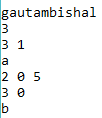
\includegraphics[scale=0.6]{assets/images/hasil.png}}
\caption{Hasil Luaran Program pada Contoh Kasus Uji Alphabetic Rope}
\label{fig:hasil-luaran}
\end{figure}

Selanjutnya dilakukan juga uji coba kebenaran dengan mengirimkan kode sumber program ke dalam situs penilaian daring SPOJ. Permasalahan yang diselesaikan adalah \problem{}. Hasil uji kebenaran dan waktu eksekusi program pada saat pengumpulan kasus uji pada situs SPOJ ditunjukkan pada Gambar \ref{figure:ujicoba}.
\begin{figure}[H]
\centerline{ 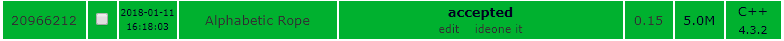
\includegraphics[scale=0.43]{assets/images/ujicoba.png}}
\caption{Hasil Uji Coba pada Situs Penilaian SPOJ}
\label{figure:ujicoba}
\end{figure}

Hal ini membuktikan bahwa implementasi yang dilakukan telah berhasil menyelesaikan \problem{} dengan batasan-batasan yang telah ditetapkan. Setelah itu dilakukan pengiriman kode sumber implementasi sebanyak 15 kali untuk melihat variasi waktu dan memori yang dibutuhkan program. Hasil uji coba sebanyak $15$ kali dapat dilihat pada Gambar \ref{figure:submission}. Grafik hasil uji coba sebanyak 15 kali ditunjukkan pada Gambar \ref{figure:grafik_spam}.
\begin{figure}[H]
\centerline{ 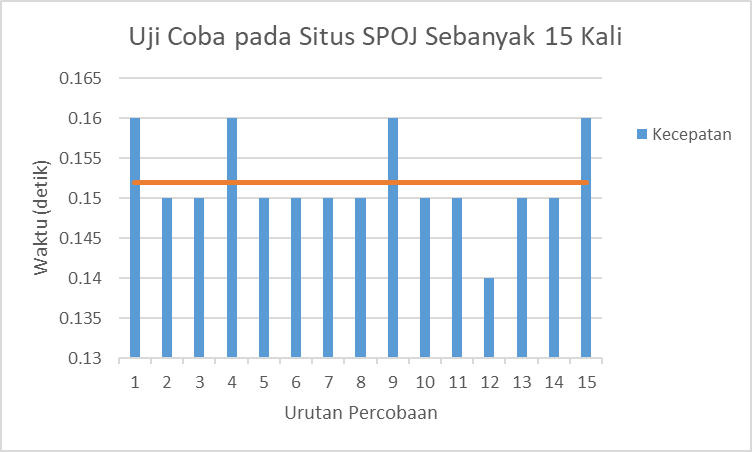
\includegraphics[scale=0.5]{assets/images/spoj-spam.png}}
\caption{Hasil Uji Coba pada Situs Penilaian SPOJ}
\label{figure:grafik_spam}
\end{figure}
\begin{table}{}
	\centering
	\begin{tabular}{|c|c|}
	\hline
		Waktu Maksimal & $0.16$ detik\\ \hline
		Waktu Minimal & $0.14$ detik\\ \hline
		Waktu Rata-Rata & $0.152$ detik\\ \hline
		Memori Maksimal & $5.0$ MB\\ \hline
		Memori Minimal & $5.0$ MB\\ \hline
		Memori Rata-rata & $5.0$ MB\\ \hline
	\end{tabular}\caption{Kecepatan Maksimal, Minimal dan Rata-Rata dari Hasil Uji Coba Sebanyak 15 Kali pada Situs Pengujian SPOJ \label{tab:pengujian}}
\end{table}
Berdasarkan Tabel \ref{tab:pengujian} dari percobaan pengujian yang dilakukan, didapat waktu rata-rata program yaitu $0.152$ detik dan penggunaan memori yang dibutuhkan program yaitu $5.0$ MB. Hasil ini masih dibawah dari batas maksimal waktu dan memori pada \problem{}, yaitu $1$ detik dan $1536$ MB.

\section{Uji Coba Kinerja}
\label{section:ujikinerja}
Uji coba kinerja penyelesaian \problem{} dilakukan dengan cara membandingkan waktu yang dibutuhkan untuk penyelesaian menggunakan \textit{string} dengan struktur data Rope yang dibuat.
\subsection{Operasi 1 Menggabungkan \textit{Rope} pada Posisi Awal}
Pada Gambar \ref{figure:operasi1string} terlihat bahwa untuk $N \gets 5000$ sampai $N \gets 10^5$ dengan banyak $Q \gets 10^5$, struktur Rope yang dibuat untuk penyelesaian \problem{} menunjukkan waktu yang lebih cepat dibandingan dengan algoritma String dan stuktur data Rope pembanding. Sedangkan untuk $N \gets 10^5$ dengan $Q \gets 5000$ sampai $Q \gets 10^5$, pertumbuhan waktu secara logaritmik dan lebih kecil dibandingkan dengan algoritma String dan struktur data Rope pembanding yang ditunjukkan pada Gambar \ref{figure:operasi1query}. Untuk tabel performa antara algoritma String dengan struktur data Rope yang telah dibuat dapat dilihat pada Tabel \ref{tab:operasi1string} dan \ref{tab:operasi1query}.
\begin{figure}
\centerline{ 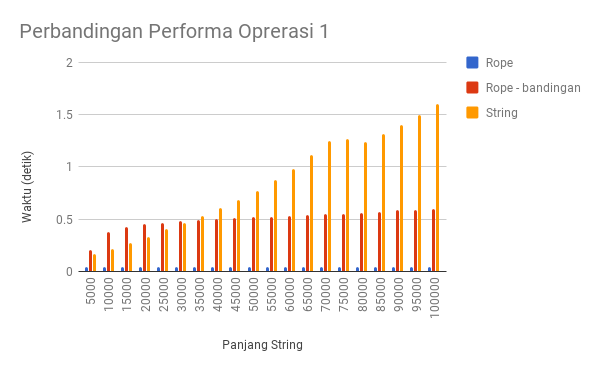
\includegraphics[scale=0.45]{assets/images/operasi1-string.png}}
\caption{Hasil Uji Coba pada Operasi 1 dengan Jumlah \textit{Query} Tetap dan Panjang \textit{String} Bertambah}
\label{figure:operasi1string}
\end{figure}

\begin{figure}
\centerline{ 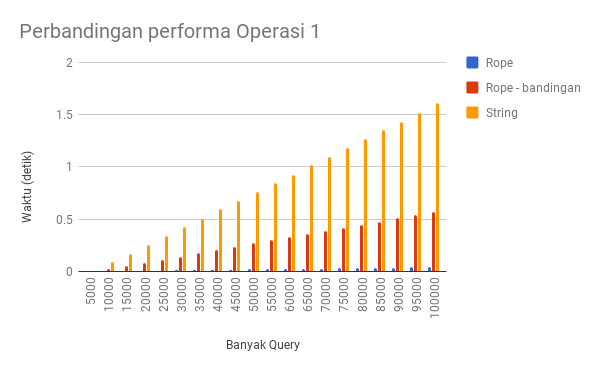
\includegraphics[scale=0.45]{assets/images/operasi1-query.png}}
\caption{Hasil Uji Coba pada Operasi 1 dengan Jumlah \textit{String} Tetap dan Jumlah \textit{Query} Bertambah}
\label{figure:operasi1query}
\end{figure}

\subsection{Operasi 2 Menggabungkan \textit{Rope} pada Posisi Akhir}
Pada Gambar \ref{figure:operasi2string} terlihat bahwa untuk $N \gets 5000$ sampai $N \gets 10^5$ dengan banyak $Q \gets 10^5$, struktur Rope yang dibuat untuk penyelesaian \problem{} menunjukkan waktu yang lebih cepat dibandingan dengan algoritma String dan stuktur data Rope pembanding. Sedangkan untuk $N \gets 10^5$ dengan $Q \gets 5000$ sampai $Q \gets 10^5$, pertumbuhan waktu secara logaritmik dan lebih kecil dibandingkan dengan algoritma String dan struktur data Rope pembanding yang ditunjukkan pada Gambar \ref{figure:operasi2query}. Untuk tabel performa antara algoritma String dengan struktur data Rope yang telah dibuat dapat dilihat pada Tabel \ref{tab:operasi2string} dan \ref{tab:operasi2query}.
\begin{figure}
\centerline{ 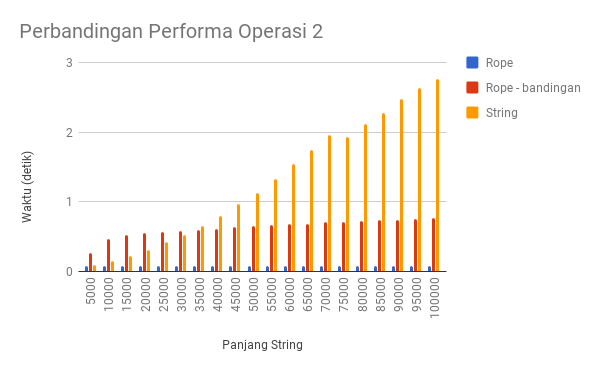
\includegraphics[scale=0.45]{assets/images/operasi2-string.png}}
\caption{Hasil Uji Coba pada Operasi 2 dengan Jumlah \textit{Query} Tetap dan Jumlah \textit{String} Bertambah}
\label{figure:operasi2string}
\end{figure}

\begin{figure}
\centerline{ 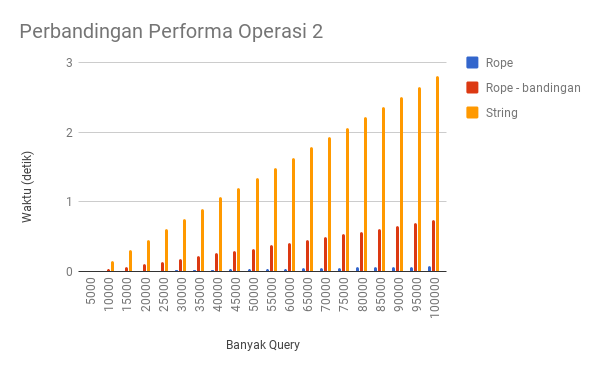
\includegraphics[scale=0.45]{assets/images/operasi2-query.png}}
\caption{Hasil Uji Coba pada Operasi 2 dengan Panjang \textit{String} Tetap dan Jumlah \textit{Query} Bertambah}
\label{figure:operasi2query}
\end{figure}

\subsection{Operasi 3 Mencetak Karakter pada Indeks ke-Y}
Pada Gambar \ref{figure:operasi3string} terlihat bahwa untuk $N \gets 5000$ sampai $N \gets 10^5$ dengan banyak $Q \gets 10^5$, algoritma String untuk penyelesaian \problem{} menunjukkan waktu yang lebih cepat dibandingan dengan struktur data Rope yang dibuat dan stuktur data Rope pembanding. Dan berlaku ketika menjalankan operasi untuk $N \gets 10^5$ dengan $Q \gets 5000$ sampai $Q \gets 10^5$ yang ditunjukkan pada Gambar \ref{figure:operasi3query}. Untuk tabel performa antara algoritma String dengan struktur data Rope yang telah dibuat dapat dilihat pada Tabel \ref{tab:operasi3string} dan \ref{tab:operasi3query}.

\begin{figure}
\centerline{ 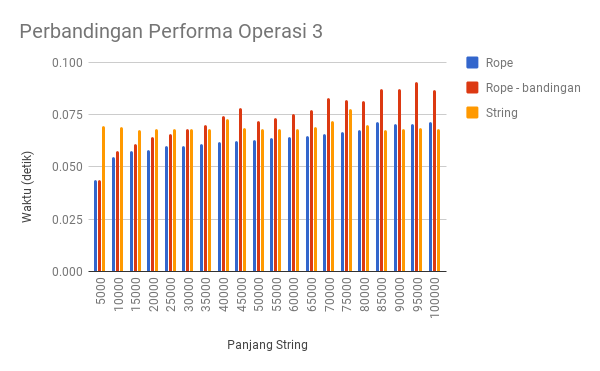
\includegraphics[scale=0.45]{assets/images/operasi3-string.png}}
\caption{Hasil Uji Coba pada Operasi 3 dengan Jumlah \textit{Query} Tetap dan Panjang \textit{String} Bertambah}
\label{figure:operasi3string}
\end{figure}

\begin{figure}
\centerline{ 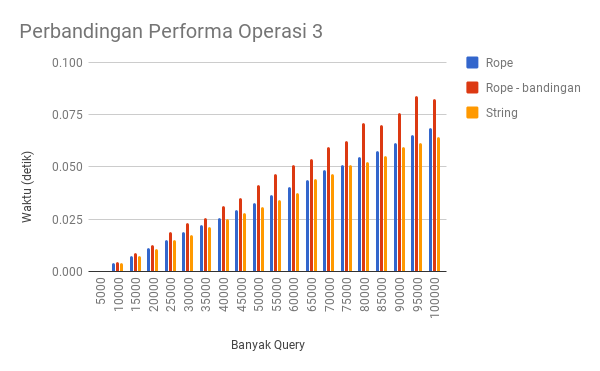
\includegraphics[scale=0.45]{assets/images/operasi3-query.png}}
\caption{Hasil Uji Coba pada Operasi 3 dengan Jumlah \textit{String} Tetap dan Jumlah \textit{Query} Bertambah}
\label{figure:operasi3query}
\end{figure}

Perbedaan \textit{rope} dengan \textit{rope}-bandingan terletak pada operasi \textit{insert}. Pada \textit{rope} bandingan operasi \textit{insert} dilakukan sama seperti algoritma \textit{insert} pada BST. Sedangkan pada \textit{rope}, \textit{insert} dilakukan dengan membagi dua panjang \textit{string} kemudian dimasukkan ke dalam \textit{tree}.

\section{Analisis Hasil Uji Coba}
Pada subbab ini akan dibahas mengenai analisis hasil uji coba yang dikerjakan pada subbab \ref{section:ujikebenaran}. Berdasarkan ketiga skenario yang telah dilakukan, masing-masing membuktikan kebenaran dan efisiensi hasil implementasi Tugas Akhir ini.\\
Dari ketiga hasil uji coba yang telah dilakukan, dapat dilihat bahwa hasil implementasi algoritma penyelesaian \problem{} pada Tugas Akhir ini mengeluarkan hasil keluaran yang sama dengan jalur yang ditelusuri secara manual. Hasil uji coba kebenaran pada subbab \ref{section:ujikebenaran} dapat digunakan sebagai acuan bahwa hasil keluaran program akan benar untuk segala jenis operasi pertanyaan dan perubahan.\\
Selanjutnya berdasarkan uji coba performa yang ditunjukkan pada Gambar \ref{figure:submission}, dapat dilihat bahwa memori dan waktu yang dibutuhkan untuk mengeksekusi program dapat dikategorikan efisien menurut situs SPOJ.\\
Proses \textit{split, concate} dan \textit{print} pada \textit{rope} mengacu pada algoritma pencarian pada \textit{tree} sehingga dapat disimpulkan bahwa kompleksitas waktu yang diperlukan sebesar $O(\log N)$. Pada proses pembuatan \textit{rope} berdasarkan Kode Sumber \ref{source:fungsi_build} didapatkan kompleksitas waktu sebesar $O(N \log N)$. Sehingga dapat disimpulkan bahwa kompleksitas waktu untuk algoritma komputasi \textit{string} pada Tugas Akhir ini adalah $O(\log N)$, dimana $N$ merupakan panjang \textit{string}. Sedangkan algoritma String membutuhkan kompleksitas sebesar $O(N)$ untuk setiap proses \textit{split} dan \textit{concate}\cite{string}.\\
Pada hasil perbandingan antara algoritma String dengan struktur Rope yang digunakan pada Tugas Akhir ini, ditunjukkan perbedaan pada kecepatan eksekusi program. Hal ini menunjukkan bahwa algoritma pada Tugas Akhir ini lebih efisien daripada algoritma String dan Rope-bandingan.
	\chapter{KESIMPULAN}

Pada bab ini dijelaskan mengenai kesimpulan dari hasil uji coba yang telah dilakukan.

\section{Kesimpulan}

Dari hasil uji coba yang telah dilakukan terhadap perancangan dan implementasi algoritma untuk menyelesaikan \problem{} dapat diambil kesimpulan sebagai berikut:

\begin{enumerate}
	\item Implementasi algoritma dengan menggunakan struktur data Rope dapat menyelesaikan \problem{} dengan benar. 
	\item Kompleksitas waktu sebesar $O(\log N)$ dapat menyelesaikan \problem{}.
	\item Waktu yang dibutuhkan program untuk menyelesaikan \problem{} minimum $0.14$ detik, maksimum $0.16$ detik dan rata-rata $0.152$ detik. Memori yang dibutuhkan sebesar $5.0$ MB.
	\item Struktur data Rope yang dibuat sangat baik diaplikasikan untuk melakukan komputasi \textit{string} yang panjang.
\end{enumerate}

\section{Saran}

Pada Tugas Akhir kali ini tentunya terdapat kekurangan serta nilai-nilai yang dapat penulis ambil. Berikut adalah saran-saran yang dapat diambil melalui Tugas Akhir ini:

\begin{enumerate}
	\item Struktur data Rope adalah pendekatan yang sesuai untuk menyelesaikan permasalahan \textit{string} yang sangat panjang.
	\item Struktur data Rope dapat diimplementasikan pada bahasa pemrograman lain.
\end{enumerate}
	
	\renewcommand\chaptername{LAMPIRAN}
	\appendix
	\begin{thebibliography}{9}
	\bibitem{arope}
	\textbf{AROPE} - Alphabetic Rope [Online]. Available: http://www.spoj.com/problems/AROPE/. [Accessed 24-October-2017].
	
	\bibitem{string}
	\textbf{Advance Programming with C++}. Available: http://www.acsu.buffalo.edu/~fineberg/mfc158/week10lecture.htm. [Accessed 24-October-2017].		
	
	\bibitem{cormen}
	T. H. Cormen, C. E. Leiserson, R. L. Rivest, and C. Stein,
	\textbf{Introduction To Algorithm,} 2nd ed. Cambridge, Massachusetts London, England: The MIT Press, 2001.
	
	\bibitem{treap}
	Cecilia R. Aragon, \textbf{Randomize Search Trees}, USA: Foundation of Computer Science, 1989.
	
	\bibitem{rope}
	Hans-J. Boehm, Russ Atkinson and Michael Pass, \textbf{Ropes: an Alternative to String}, California: Xeroc PARC, 1994.
		
\end{thebibliography}

	\begin{appendices}

  \chapter{Hasil Uji Coba Kebenaran pada Situs SPOJ}
  \setcounter{figure}{0}
  \renewcommand{\thetable}{A.\arabic{table}}
  \renewcommand{\thefigure}{A.\arabic{figure}}
  
  \begin{figure}[H]
  	\centerline{ 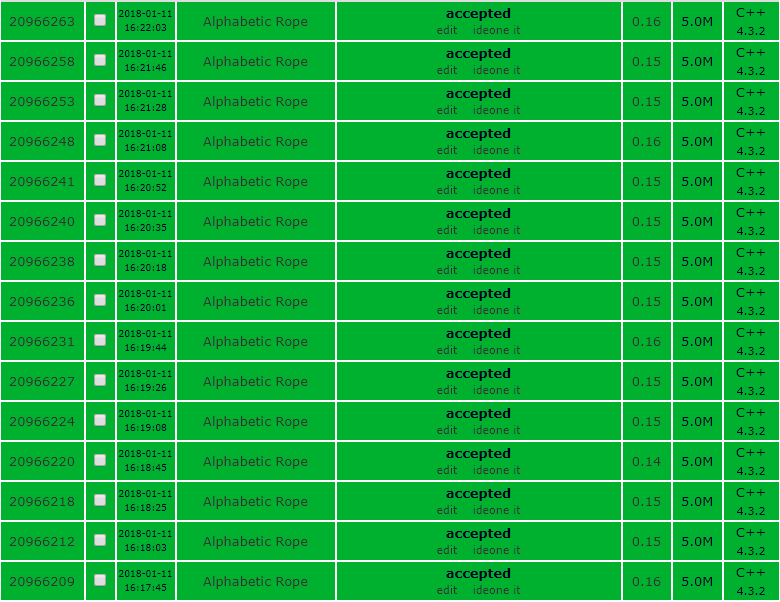
\includegraphics[scale=0.5]{assets/images/submission.png}}
  	\caption{Hasil Pengujian Sebanyak 15 Kali pada Situs Penilaian Daring SPOJ}
  	\label{figure:submission}
  \end{figure}
  
  \chapter{Hasil Uji Performa Penyelesaian Operasi 1 Menggunakan Struktur Data Rope dan Algorithma String}
  \setcounter{figure}{0}
  \renewcommand{\thetable}{B.\arabic{table}}
  \renewcommand{\thefigure}{B.\arabic{figure}}
  
  \begin{table} [H]
  \centering
	  \begin{tabular}{|c|c|c|c|}
		  \hline
		  \multirow{2}{*}{Panjang String} & Rope & Rope - pembanding & String\\
		  		  & Waktu (detik) & Waktu (detik) & Waktu (detik)\\ \hline
		  5000 & 0.04584	& 0.37512	& 0.21461\\ \hline
		  10000 & 0.04568	& 0.42488	& 0.27259\\ \hline
		  15000 & 0.04298	& 0.45005	& 0.32707\\ \hline
		  20000 & 0.04261	& 0.46458	& 0.40244\\ \hline
		  25000 & 0.04352	& 0.47984	& 0.46670\\ \hline
		  30000 & 0.04239	& 0.48971	& 0.53264\\ \hline
		  35000 & 0.04229	& 0.49920	& 0.60791\\ \hline
		  40000 & 0.04324	& 0.50714	& 0.68570\\ \hline
		  45000 & 0.04716	& 0.51634	& 0.77109\\ \hline
		  50000 & 0.04239	& 0.52379	& 0.87648\\ \hline
		  55000 & 0.04225	& 0.53031	& 0.98290\\ \hline
		  60000 & 0.04218	& 0.53815	& 1.11034\\ \hline
		  65000 & 0.04262	& 0.54562	& 1.24909\\ \hline
		  70000 & 0.04251	& 0.55366	& 1.26256\\ \hline
		  75000 & 0.04286	& 0.56215	& 1.24042\\ \hline
		  80000 & 0.04524	& 0.57252	& 1.31375\\ \hline
		  85000 & 0.04271	& 0.58538	& 1.40470\\ \hline
		  90000 & 0.04243	& 0.58756	& 1.49502\\ \hline
		  95000 & 0.04246	& 0.60007	& 1.59853\\ \hline
		  100000 & 0.04229	& 0.60352	& 1.69388\\ \hline
	  \end{tabular}\caption{Tabel Hasil Uji Coba pada Operasi 1 dengan Jumlah \textit{Query} tetap dan Panjang \textit{String} Bertambah}
	  \label{tab:operasi1string}
  \end{table}
  
  \begin{table} [H]
    \centering
  	  \begin{tabular}{|c|c|c|c|}
  		  \hline
  		  \multirow{2}{*}{Banyak Query} & Rope & Rope - pembanding & String\\
  		    		  & Waktu (detik) & Waktu (detik) & Waktu (detik)\\ \hline
  		  5000	& 0.00212	& 0.02678	& 0.09447\\ \hline
  		  10000	& 0.00426	& 0.05573	& 0.17078\\ \hline
  		  15000	& 0.00634	& 0.08553	& 0.25521\\ \hline
  		  20000	& 0.00851	& 0.11321	& 0.33912\\ \hline
  		  25000	& 0.01048	& 0.14259	& 0.42499\\ \hline
  		  30000	& 0.01272	& 0.17272	& 0.50647\\ \hline
  		  35000	& 0.01482	& 0.20204	& 0.59519\\ \hline
  		  40000	& 0.01777	& 0.23304	& 0.67729\\ \hline
  		  45000	& 0.01924	& 0.27471	& 0.75871\\ \hline
  		  50000	& 0.02168	& 0.29658	& 0.84541\\ \hline
  		  55000	& 0.02483	& 0.32535	& 0.92717\\ \hline
  		  60000	& 0.02616	& 0.3547	& 1.01493\\ \hline
  		  65000	& 0.02785	& 0.38604	& 1.09944\\ \hline
  		  70000	& 0.02959	& 0.41976	& 1.18202\\ \hline
  		  75000	& 0.03220	& 0.44713	& 1.26605\\ \hline
  		  80000	& 0.03432	& 0.47656	& 1.35644\\ \hline
  		  85000	& 0.03614	& 0.50967	& 1.43311\\ \hline
  		  90000	& 0.03923	& 0.53864	& 1.51598\\ \hline
  		  95000	& 0.04044	& 0.56934	& 1.60935\\ \hline
  		  100000	& 0.04229	& 0.60352	& 1.69388\\ \hline
  	  \end{tabular}\caption{Tabel Hasil Uji Coba pada Operasi 1 dengan Panjang \textit{String} tetap dan Jumlah \textit{Query} Bertambah}
  	  \label{tab:operasi1query}
    \end{table}
    
  \chapter{Hasil Uji Performa Penyelesaian Operasi 2 Menggunakan Struktur Data Rope dan String}
  \setcounter{figure}{0}
  \renewcommand{\thetable}{C.\arabic{table}}
  \renewcommand{\thefigure}{C.\arabic{figure}}
  
  \begin{table}[h]
  \centering
	  \begin{tabular}{|c|c|c|c|}
		  \hline
		  \multirow{2}{*}{Panjang String} & Rope & Rope - pembanding & String\\
		  		  & Waktu (detik) & Waktu (detik) & Waktu (detik)\\ \hline
		  5000	& 0.08046	& 0.45924	& 0.15061\\ \hline
		  10000	& 0.07907	& 0.51843	& 0.21968\\ \hline
		  15000	& 0.07804	& 0.54997	& 0.30699\\ \hline
		  20000	& 0.07941	& 0.56391	& 0.42457\\ \hline
		  25000	& 0.07919	& 0.58758	& 0.52275\\ \hline
		  30000	& 0.08137	& 0.59856	& 0.64959\\ \hline
		  35000	& 0.07963	& 0.6151	& 0.80127\\ \hline
		  40000	& 0.0807	& 0.6351	& 0.96337\\ \hline
		  45000	& 0.07853	& 0.64935	& 1.12678\\ \hline
		  50000	& 0.07917	& 0.66312	& 1.33048\\ \hline
		  55000	& 0.08274	& 0.67976	& 1.5374\\ \hline
		  60000	& 0.07855	& 0.68753	& 1.74437\\ \hline
		  65000	& 0.07848	& 0.70459	& 1.9582\\ \hline
		  70000	& 0.08031	& 0.71008	& 1.93652\\ \hline
		  75000	& 0.07816	& 0.73011	& 2.12236\\ \hline
		  80000	& 0.07947	& 0.73807	& 2.27391\\ \hline
		  85000	& 0.08009	& 0.7404	& 2.4679\\ \hline
		  90000	& 0.07838	& 0.74922	& 2.63696\\ \hline
		  95000	& 0.07819	& 0.76165	& 2.7606\\ \hline
		  100000	& 0.08379	& 0.76779	& 2.94229\\ \hline
	  \end{tabular}\caption{Tabel Hasil Uji Coba pada Operasi 2 dengan Jumlah \textit{Query} tetap dan Panjang \textit{String} Bertambah}
	  \label{tab:operasi2string}
  \end{table}
  
  \begin{table}[h]
    \centering
  	  \begin{tabular}{|c|c|c|c|}
 		  \hline
 		  \multirow{2}{*}{Banyak Query} & Rope & Rope - pembanding & String\\
 		    		  & Waktu (detik) & Waktu (detik) & Waktu (detik)\\ \hline
  		  5000	& 0.0021	& 0.03094	& 0.15582\\ \hline
  		  10000	& 0.00422	& 0.06923	& 0.31249\\ \hline
  		  15000	& 0.0082	& 0.10347	& 0.45776\\ \hline
  		  20000	& 0.01235	& 0.14144	& 0.60343\\ \hline
  		  25000	& 0.01652	& 0.17569	& 0.75053\\ \hline
  		  30000	& 0.02187	& 0.21542	& 0.89214\\ \hline
  		  35000	& 0.02437	& 0.25814	& 1.06315\\ \hline
  		  40000	& 0.02868	& 0.29264	& 1.19422\\ \hline
  		  45000	& 0.03337	& 0.32757	& 1.33897\\ \hline
  		  50000	& 0.03724	& 0.37407	& 1.48473\\ \hline
  		  55000	& 0.04161	& 0.41413	& 1.62678\\ \hline
  		  60000	& 0.04647	& 0.45708	& 1.77913\\ \hline
  		  65000	& 0.04975	& 0.48762	& 1.92705\\ \hline
  		  70000	& 0.05391	& 0.5315	& 2.06298\\ \hline
  		  75000	& 0.05869	& 0.57248	& 2.21603\\ \hline
  		  80000	& 0.06229	& 0.61257	& 2.35933\\ \hline
  		  85000	& 0.06674	& 0.65026	& 2.50408\\ \hline
  		  90000	& 0.07095	& 0.68927	& 2.64912\\ \hline
  		  95000	& 0.07366	& 0.74459	& 2.80072\\ \hline
  		  100000	& 0.08379	& 0.76779	& 2.94229\\ \hline
  	  \end{tabular}\caption{Tabel Hasil Uji Coba pada Operasi 2 dengan Panjang String tetap dan Jumlah Query Bertambah}
  	  \label{tab:operasi2query}
    \end{table}
    
  \chapter{Hasil Uji Performa Penyelesaian Operasi 3 Menggunakan Struktur Data Rope dan String}
  \setcounter{figure}{0}
  \renewcommand{\thetable}{D.\arabic{table}}
  \renewcommand{\thefigure}{D.\arabic{figure}}
  
  \begin{table}[h]
  \centering
	 \begin{tabular}{|c|c|c|c|}
		  \hline
		  \multirow{2}{*}{Panjang String} & Rope & Rope - pembanding & String\\
		  		  & Waktu (detik) & Waktu (detik) & Waktu (detik)\\ \hline
		  5000	& 0.05484	& 0.05753	& 0.06929\\ \hline
		  10000	& 0.05765	& 0.06085	& 0.06749\\ \hline
		  15000	& 0.05815	& 0.06444	& 0.06798\\ \hline
		  20000	& 0.06014	& 0.06593	& 0.06812\\ \hline
		  25000	& 0.06007	& 0.06808	& 0.06819\\ \hline
		  30000	& 0.06121	& 0.06983	& 0.06805\\ \hline
		  35000	& 0.06197	& 0.07425	& 0.07311\\ \hline
		  40000	& 0.06253	& 0.0781	& 0.06874\\ \hline
		  45000	& 0.06310	& 0.07199	& 0.06835\\ \hline
		  50000	& 0.06381	& 0.0733	& 0.06814\\ \hline
		  55000	& 0.06449	& 0.07532	& 0.06797\\ \hline
		  60000	& 0.06485	& 0.07707	& 0.0689\\ \hline
		  65000	& 0.06592	& 0.08287	& 0.07186\\ \hline
		  70000	& 0.06668	& 0.08182	& 0.07765\\ \hline
		  75000	& 0.06788	& 0.08158	& 0.06994\\ \hline
		  80000	& 0.07156	& 0.08723	& 0.06788\\ \hline
		  85000	& 0.07049	& 0.0875	& 0.06823\\ \hline
		  90000	& 0.07054	& 0.09047	& 0.06874\\ \hline
		  95000	& 0.07153	& 0.08684	& 0.06834\\ \hline
		  100000	& 0.07222	& 0.0871	& 0.07223\\ \hline
	  \end{tabular}\caption{Tabel Hasil Uji Coba pada Operasi 3 dengan Jumlah \textit{Query} tetap dan Panjang \textit{String} Bertambah}
	  \label{tab:operasi3string}
  \end{table}
  
  \begin{table}[h]
    \centering
  	  \begin{tabular}{|c|c|c|c|}
   		  \hline
   		  \multirow{2}{*}{Banyak Query} & Rope & Rope - pembanding & String\\
   		    		  & Waktu (detik) & Waktu (detik) & Waktu (detik)\\ \hline
  		  5000	& 0.00403	& 0.0046	& 0.00411\\ \hline
  		  10000	& 0.00753	& 0.00901	& 0.00729\\ \hline
  		  15000	& 0.01116	& 0.01278	& 0.01078\\ \hline
  		  20000	& 0.01524	& 0.01901	& 0.01501\\ \hline
  		  25000	& 0.01878	& 0.02309	& 0.01763\\ \hline
  		  30000	& 0.02204	& 0.02543	& 0.02134\\ \hline
  		  35000	& 0.02565	& 0.03114	& 0.02496\\ \hline
  		  40000	& 0.02920	& 0.03496	& 0.02786\\ \hline
  		  45000	& 0.03271	& 0.04112	& 0.03096\\ \hline
  		  50000	& 0.03638	& 0.04661	& 0.03399\\ \hline
  		  55000	& 0.04029	& 0.05072	& 0.03738\\ \hline
  		  60000	& 0.04361	& 0.05377	& 0.04412\\ \hline
  		  65000	& 0.04844	& 0.05963	& 0.04669\\ \hline
  		  70000	& 0.05078	& 0.06232	& 0.05085\\ \hline
  		  75000	& 0.05493	& 0.07118	& 0.05242\\ \hline
  		  80000	& 0.05782	& 0.06998	& 0.05502\\ \hline
  		  85000	& 0.06153	& 0.0758	& 0.05955\\ \hline
  		  90000	& 0.06514	& 0.08392	& 0.06156\\ \hline
  		  95000	& 0.06884	& 0.08232	& 0.06455\\ \hline
  		  100000	& 0.07222	& 0.0871	& 0.07223\\ \hline
  	  \end{tabular}\caption{Tabel Hasil Uji Coba pada Operasi 3 dengan Panjang String tetap dan Jumlah Query Bertambah}
  	  \label{tab:operasi3query}
    \end{table}

\end{appendices}
	\backmatter
	\chapter{BIODATA PENULIS}
\begin{wrapfigure}{l}{0.3\textwidth}
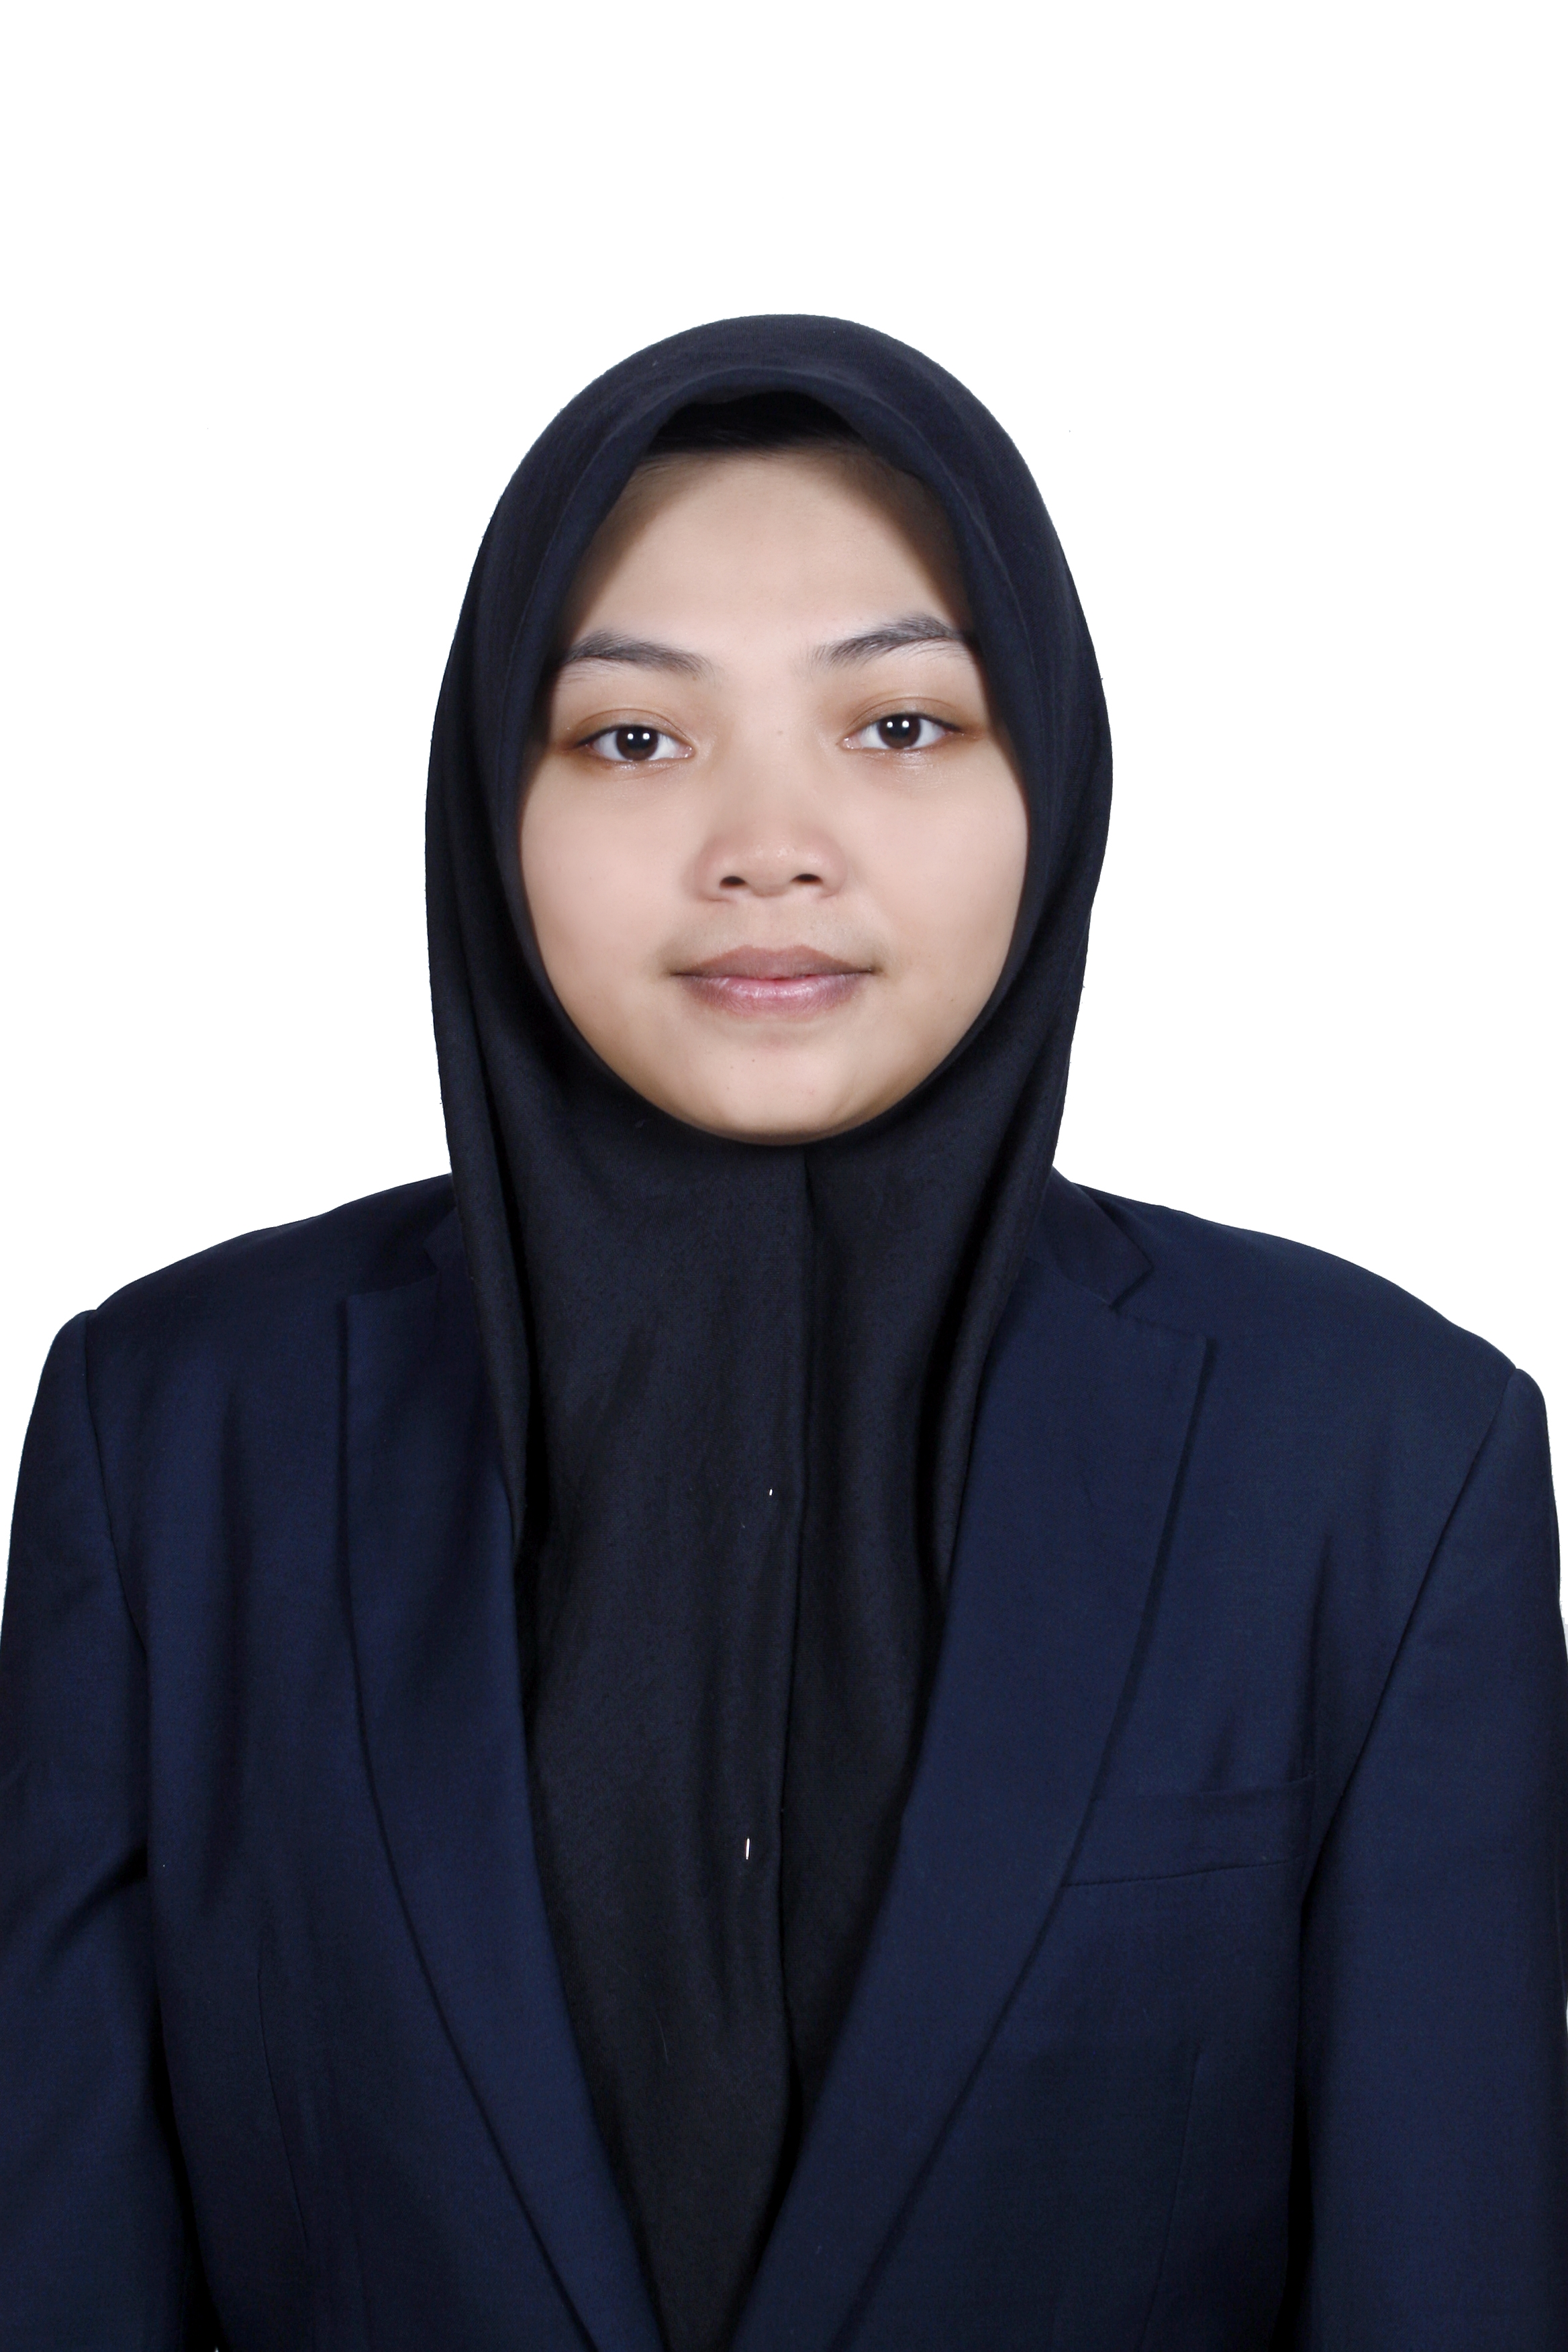
\includegraphics[height=0.3\textheight]{biodata/foto.JPG}
\end{wrapfigure}

\textbf{Desy Nurbaiti Rahmi}, lahir di Banyuwangi tanggal 9 Desember 1995. Penulis merupakan anak ketiga dari 3 bersaudara. Penulis telah menempuh pendidikan formal TK Aisyiyah I Banyuwangi, SD Negeri 1 Kebalenan (2002-2008), SMP Negeri 1 Banyuwangi (2008-2011) dan SMA Negeri 1 Glagah (2011-2014). Penulis melanjutkan studi kuliah program sarjana di Jurusan Teknik Informatika ITS. 

Selama kuliah di Teknik Informatika ITS, penulis  pernah menjadi asisten dosen dan praktikum untuk mata kuliah Sistem Operasi (2016 dan 2017), Jaringan Komputer(2016). Selama menempuh perkuliahan penulis juga aktif di kegiatan organisasi dan kepanitiaan diantaranya menjadi staff Departemen Pengembangan Profesi HMTC ITS, wakil dua Bendahara Schematics 2015, Bendahara Schematics 2015 dan panitia Pemusatan Latihan Nasional 2 TOKI 2017 di ITS. Penulis dapat dihubungi melalui surel di \\ \texttt{desyrahmi09@gmail.com}.

\end{document}
